%%%%%%%%%%%%%%%%%%%%%%%%%%%%%%%%%%%%%%%%%
% Masters/Doctoral Thesis 
% LaTeX Template
% Version 2.5 (27/8/17)
%
% This template was downloaded from:
% http://www.LaTeXTemplates.com
%
% Version 2.x major modifications by:
% Vel (vel@latextemplates.com)
%
% This template is based on a template by:
% Steve Gunn (http://users.ecs.soton.ac.uk/srg/softwaretools/document/templates/)
% Sunil Patel (http://www.sunilpatel.co.uk/thesis-template/)
%
% Template license:
% CC BY-NC-SA 3.0 (http://creativecommons.org/licenses/by-nc-sa/3.0/)
%
%%%%%%%%%%%%%%%%%%%%%%%%%%%%%%%%%%%%%%%%%

%----------------------------------------------------------------------------------------
%	PACKAGES AND OTHER DOCUMENT CONFIGURATIONS
%----------------------------------------------------------------------------------------

\documentclass[
11pt, % The default document font size, options: 10pt, 11pt, 12pt
%oneside, % Two side (alternating margins) for binding by default, uncomment to switch to one side
english, % ngerman for German
singlespacing, % Single line spacing, alternatives: onehalfspacing or doublespacing
%draft, % Uncomment to enable draft mode (no pictures, no links, overfull hboxes indicated)
%nolistspacing, % If the document is onehalfspacing or doublespacing, uncomment this to set spacing in lists to single
%liststotoc, % Uncomment to add the list of figures/tables/etc to the table of contents
%toctotoc, % Uncomment to add the main table of contents to the table of contents
%parskip, % Uncomment to add space between paragraphs
%nohyperref, % Uncomment to not load the hyperref package
headsepline, % Uncomment to get a line under the header
%chapterinoneline, % Uncomment to place the chapter title next to the number on one line
%consistentlayout, % Uncomment to 
change the layout of the declaration, abstract and acknowledgements pages to match the default layout
]{MastersDoctoralThesis} % The class file specifying the document structure

\usepackage[utf8]{inputenc} % Required for inputting international characters
\usepackage[T1]{fontenc} % Output font encoding for international characters
\usepackage{tikz}
\usepackage{mathpazo} % Use the Palatino font by default
\usepackage[bottom]{footmisc}

\usepackage[backend=bibtex,style=authoryear,natbib=true]{biblatex} % Use the bibtex backend with the authoryear citation style (which resembles APA)
\addbibresource{references.bib} % The filename of the bibliography

\usepackage[autostyle=true]{csquotes} % Required to generate language-dependent quotes in the bibliography

\usepackage{amsmath}
\usepackage{listings}
\usepackage{color}

\usepackage{algorithm}% http://ctan.org/pkg/algorithms
\usepackage{algpseudocode}% http://ctan.org/pkg/algorithmicx
\algtext*{EndIf}
\algtext*{EndFor}

\definecolor{codegreen}{rgb}{0,0.6,0}
\definecolor{codegray}{rgb}{0.5,0.5,0.5}
\definecolor{codepurple}{rgb}{0.58,0,0.82}
\definecolor{backcolour}{rgb}{0.95,0.95,0.92}
\definecolor{keywordred}{HTML}{ba3030}
\definecolor{charclasspurple}{HTML}{a52b70}
\definecolor{operatordark}{HTML}{683ba0}

 
\lstdefinestyle{highlighter}{
    backgroundcolor=\color{backcolour},   
    commentstyle=\color{codegreen},
    keywordstyle=\color{magenta},
    numberstyle=\tiny\color{codegray},
    stringstyle=\color{codepurple},
    basicstyle=\ttfamily\small,
    breakatwhitespace=false,         
    breaklines=true,                 
    captionpos=b,                    
    keepspaces=true,                 
    numbers=left,                    
    numbersep=5pt,                  
    showspaces=false,                
    showstringspaces=false,
    showtabs=false,                  
    tabsize=2
}
\lstdefinelanguage{RascalGrammar}
{
  keywords={start,lexical,syntax,layout,keyword,bracket,left,right,non-assoc, assoc},
  classoffset=1, % starting new class
  otherkeywords={>>,!>>,!<<,<<,\\},
  morekeywords={>>,!>>,!<<,<<,\\},
  keywordstyle=\color{keywordred},
  classoffset=0,
  comment=[l]{//},
  morecomment=[s]{/*}{*/},
  morecomment=[l]{@},
  string=[bd]",
  morestring=[bd]',
  moredelim=[s][\color{charclasspurple}]{\[}{\]},
  columns=flexible,
  keepspaces=true,
  showstringspaces=false,
  basicstyle=\ttfamily\small,
  commentstyle=\color{codegreen},
  keywordstyle=\color{keywordred},
  stringstyle=\color{codepurple}
}
 
\lstdefinelanguage{Rascal}
{
  language=Java,
  morekeywords={data,list,bool,set,str,map,int,real,rel,tuple,alias},
  classoffset=2, % starting new class
  keywords={Symbol,Condition,CharRange,Attr,Associativity,Production},
%  morekeywords={Symbol,Condition,CharRange,Attr,Associativity,Production},
  keywordstyle=\color{charclasspurple},
  classoffset=0,
  columns=flexible,
  keepspaces=true,
  showstringspaces=false,
  basicstyle=\ttfamily\small,
  commentstyle=\color{codegreen},
  keywordstyle=\color{keywordred},
  stringstyle=\color{codepurple}
}
 

\lstdefinelanguage{SublimeSyntax}
{
  keywords={contexts,variables,file_extensions,name,include,match,pop,set,push},
  classoffset=1, % starting new class
  otherkeywords={meta,true,false,scope},
  morekeywords={meta,true,false,scope},
  keywordstyle=\color{cyan},
  classoffset=0,
  comment=[l]{\#},
  morecomment=[l]{\%},
  morestring=[bd]",
  morestring=[bd]',
  columns=flexible,
  keepspaces=true,
  showstringspaces=false,
  basicstyle=\ttfamily,
  commentstyle=\color{codegreen},
  keywordstyle=\color{keywordred},
  stringstyle=\color{codepurple}
} 

\newcommand{\gram}[1]{\lstinline[language=RascalGrammar, basicstyle=\normalsize\ttfamily]|#1|} 
\newcommand{\data}[1]{\lstinline[language=Rascal, basicstyle=\normalsize\ttfamily]|#1|}

\lstset{style=highlighter, language=Rascal}

%----------------------------------------------------------------------------------------
%	MARGIN SETTINGS
%----------------------------------------------------------------------------------------
%
\geometry{
	paper=a4paper, % Change to letterpaper for US letter
	inner=2.5cm, % Inner margin
	outer=3.8cm, % Outer margin
	bindingoffset=.5cm, % Binding offset
	top=1.5cm, % Top margin
	bottom=1.5cm, % Bottom margin
	%showframe, % Uncomment to show how the type block is set on the page
}

%----------------------------------------------------------------------------------------

% Define some commands to keep the formatting separated from the content 
\newcommand{\keyword}[1]{\textbf{#1}}
\newcommand{\tabhead}[1]{\textbf{#1}}
\newcommand{\code}[1]{\texttt{#1}}
\newcommand{\file}[1]{\texttt{\bfseries#1}}
\newcommand{\option}[1]{\texttt{\itshape#1}}

\newcommand{\prodgr}[2]{#1 \rightarrow #2}
\newcommand{\prodstar}[2]{#1 \rightarrow^* #2}
\newcommand{\prodeps}[1]{#1 \rightarrow \epsilon}

\newcommand{\alprod}[2]{#1 &\rightarrow #2}
\newcommand{\alprodstar}[2]{#1 &\rightarrow^* #2}
\newcommand{\alprodeps}[1]{#1 &\rightarrow \epsilon}



%opening
\title{test}
\author{edser}

\begin{document}

\maketitle


% Problem Description

\chapter{Project Description} % Main chapter title

\label{problemdescription} % For referencing the chapter elsewhere, use \ref{} 

%----------------------------------------------------------------------------------------

\section{Introduction}
Developers all over the world use their favourite editors in order to  software. One of the things all these editors tend to have in common is support for syntax highlighting. Syntax highlighting is the process of colouring certain words or sections of text in a document in order to give visual meaning to them. This is useful since humans can easily identify things by colour and the colours give an overall more structured look to an otherwise plain looking text document. Creating programs that do this highlighting for us is a development task in its own. The syntax highlighters tend to use (some form of) the underlying mathematical formalism of a programming language called the Context-Free-Grammar of this language. This is necessary in order to generate correct context-aware highlights. There are different forms of syntax-highlighters, some work with states and a simple stack much like finite state machines. Others, like the Rascal highlighter in Eclipse, use the Grammar and its parse-trees directly. Just as regular languages can not express everything context-free languages can, state-based highlighters cannot express everything that the context-free languages can. Hence, a translation step is needed.

\pagebreak

\section{Problem Definition}
Creating state-based syntax highlighters for different languages is a repetitive and seemingly similar process. Many editors (e.g., VS Code, Textmate, SublimeText, Atom, ACE, CodeMirror etc.) use some implementation of these state-based highlighters. This thesis is focused on generating such highlighters from the context-free definition of the language. As suggested by my supervisor I took an algorithm for transforming a context-free grammar to a regular approximation as a starting point \parencite{MohriNederhof}. From here on this thesis will describe how to solve the following question. 

\begin{center}\emph{\large How can we derive state-based highlighters from context-free grammars?}\end{center}
The algorithm was written for Rascal and this thesis will use Rascal as the main tool to fit the algorithm to, however it is described in a general way such that it is extendable to different languages. The ultimate goal would be to be able to generate a proper highlighter for Rascal's own grammar. Which contains close to all special things you can do with Rascal's grammar formalism. A second important portion of the goal is to be able to deal with tougher highlighting tasks like nested comments and string interpolation.

\subsection{Steps} \label{sec:problemdef:sub}
In order to tackle this problem the main question is divided in a number of subquestions. Each being fairly detachable from the problem as a whole, but contributing to the final result when joined with the rest.

\begin{enumerate}
	\item[\textit{1.}] How to embed highlighting information in a context-free grammar?
	\item[\textit{2.}] Can a Rascal grammar be written as the standard 4-element tuple?
	\item[\textit{3.}] How to convert a context-free grammar to a regular grammar approximating the same language?
	\item[\textit{4.}] How to create useful state-machines from these approximations?
	\item[\textit{5.}] How to map these machines to an actual state-based syntax highlighter?
\end{enumerate}

\subsection{Performance}
The designed algorithm is build logically and works for relatively simple cases. Once larger grammars and more difficult cases are tested a certain number of errors become apparent. The origin of these errors are identified and methods to avoid them are presented where possible.

% Background Information

\chapter{Background Information} % Main chapter title

\label{chap:Background} % For referencing the chapter elsewhere, use \ref{Background} 


%----------------------------------------------------------------------------------------

\section{Graph}
	\subsection{Definition}
	A graph is defined as a structure with a set of nodes called vertices ($V$) and a set of links between these nodes called edges ($E$). By this definition a graph ($G$) becomes a two-element tuple of the following form.
	\begin{equation} G = (V, E) \end{equation}	
	Traversing a graph from some vertex $v1$ to some $v2$ along the edge $(v1, v2)$ is written as:
	\begin{equation} v1 \stackrel{(v1, v2)}{\to} v2 \end{equation}
	A path with an arbitrary number of edge-traversals leading from $v1$ to $v2$ is written as:
	\begin{equation} v1 \to^* v2 \end{equation}
	
	\subsection{Strongly Connected Components}
	A directed graph is said to be \emph{strongly connected} if every vertex $v \in V$ is reachable from any other vertex $v2 \in V$. Here $v1$ and $v2$ can be the same vertex.
	\begin{equation}v1, v2 \in V : \prodstar{v1}{v2}\end{equation}
	The set of \emph{\textbf{strongly connected components}} of a directed graph $G$ is defined as the partitioning of $G$ into smaller graphs, such that all of these subgraphs are strongly connected.
	\begin{figure}[h]
		\centering
		\includegraphics[scale=0.6]{Figures/components.png}
		\decoRule
	 	\caption[Strongly connected components]{The strongly connected components of a graph}
	 	\label{fig:GraphExample}
	\end{figure}
	
		\subsubsection{Kosaraju's algorithm}
		\label{sec:Kosaraju}
		Numerous algorithms for computing the strongly connected components of a directed graph exist. Most of these also have nice time-complexities. Kosaraju's algorithm works in $\mathcal{O}(V+E)$. Officially published by \parencite{Kosaraju}, it uses the property of the inverse of a directed graph having the same strongly connected components as the original graph. Below follows a brief description of the algorithm. A few things beforehand:
		
		\begin{enumerate}
			\item A component is represented by assigning every vertex a root vertex of its component.
			\item The algorithm requires an ordered list $L$ of vertices. It will grow to contain each vertex once.
		\end{enumerate}
		The algorithm then becomes:
		\begin{enumerate}
			\item For each vertex $u \in V$, mark $u$ as unvisited. let $L$ be empty.
			\item For every vertex $u \in V$ $Visit(u)$, where $Visit(u)$ is:
				\subitem if $u$ is unvisited:
					\subsubitem Mark $u$ as visited
					\subsubitem For each out-neighbour $v$ of $u$, $Visit(v)$
					\subsubitem Prepend $u$ to $L$
			\item For each element $u$ in $L$ (in order), $Assign(u,u)$, where $Assign(u,root)$ is:
				\subitem If $u$ has not been assigned to a component:
					\subsubitem Assign $u$ as beloging to the component whose root is $root$
					\subsubitem For each in-neighbour $v$ of $u$, do $Assign(v, root)$
		\end{enumerate}
		
		
		
	\pagebreak
	
\section{Context-Free Grammar}
	\subsection{Definition}	\label{sec:CFG_def}
	A context-free grammar ($CFG$) is a 4-element tuple. It has two disjoint alphabets $V$ and $\Sigma$, a set of production rules $P$ and a startsymbol $S \in V$. A production rule $p$ is a pair $(A, w)$ with $A \in V$ and $w \in (V \cup \Sigma)^*$. The set $\Sigma$ is the set of terminals and $V$ the set of non-terminals. Empty sentences are defined by $\epsilon$\\
	\begin{equation} CFG = (V, \Sigma, P, S) \end{equation}	
	\begin{equation} p \in P, A \in V, A \rightarrow w \in (V \cup \Sigma)^*\end{equation}	
			
	\subsection{Graph of a CFG} \label{eqn:gram2graph}
	The graph of a context-free grammar is defined as follows. It is a directed graph with vertices for each non-terminal in $CFG$ and an edge from a non-terminal $A \in V$ to some other $B \in V$ iff $B$ is in $w$ for some production rule $A \rightarrow w$.
	\begin{align} 
	\vspace{-0.3in}
	\nonumber CFG &= (V_{cfg}, \Sigma, P, S)\\
	\vspace{0.1in}
	\nonumber E &= \{(A, B) | (A \rightarrow w) \in P, B \in w, B \in V_{cfg}\}\\
	\vspace{0.1in}
	G &= (V_{cfg}, E)
	\end{align}
		
	\subsection{Strongly Regular Grammars}
	\label{sec:MohriNederhof}
	Normal context-free grammars can generate languages that are not regular. In other words, these can not be mapped to equivalent finite state machines. The subclass of grammar called \emph{strongly regular grammars} are the set of grammars guaranteed to generate regular languages. This set is also the set of grammar without self-embedding \parencite{Chomsky1959}.\\\\
	Strongly regular grammars are grammars in which the rules of each set $M$ of mutually recursive nonterminals are either all right-linear or all left-linear. All non-terminals $T \not \in M$ are considered terminals here. For the sake of this thesis I chose to use the case of right-linear grammars and rewrite all conflicting rules to right-linear ones. \cite{MohriNederhof} describe a simple transformation to transform any grammar into a strongly regular one. The new grammar accepts a superset of the language of the original grammar.
	\pagebreak
	\begin{enumerate}
		\item Identify all sets $M$ of \textit{mutually recursive non-terminals}\footnote{This coincides with the strongly connected components of the grammar} such that not all\\ $p:(\prodgr{A}{w}), A \in M$ are right- or left-linear with respect to other elements of $M$.
		\item For all non-terminals with conflicting productions $A \in M, p:(\prodgr{A}{w})$ introduce a new non-terminal $A' \not \in V$. 
		\item If $A$ is directly reachable from some other non-terminal $X \not \in M$ introduce a rule $\prodeps{A'}$.
		\item For all rules with left hand side $A \in M$:
		\subitem $\prodgr{A}{\alpha_0 B_1 \alpha_1 B_2 \dots \alpha_m B_m}\vspace{0.1in}$\\
		with $m \geq 0, B_1, \dots, B_m \in M, \alpha_0, \ldots, \alpha_m \in (\Sigma \cup (N - M))^*$. Replace with:
		\begin{align}
		\nonumber \alprod{A}{\alpha_0 B_1}
		\\\nonumber \alprod{B'_1}{\alpha_1 B_2}
		\\\nonumber \alprod{B'_2}{\alpha_2 B_3}
		\\\nonumber &\ldots
		\\\nonumber \alprod{B'_{m-1}}{\alpha_{m-1} B_m}
		\\\nonumber \alprod{B'_m}{\alpha_m A'}
		\end{align}
		\item if $m = 0$, we end up with just $\prodgr{A}{\alpha_0 A'}$.					
	\end{enumerate}
	This transformation ensures that all rules of the grammar become right- or left-linear with respect to their set of recursively reachable symbols. This ensures a regular grammar and therefore that it is possible to convert this new grammar into state machines

\pagebreak

\section{State Machines}
	\subsection{Definition}
		A deterministic finite state machine (DFSM or DFA) $S$ is a 5-element tuple with a set of states ($Q$), an alphabet ($\Sigma$), an initial state ($q_0 \in Q$), a set of final states ($F \subseteq Q$) and a transition function ($\delta : (Q \times \Sigma \rightarrow Q)$) describing how to move from one state to the next. Alongside this we define a transition as a 3-element tuple.
		\begin{equation} S = (Q, \Sigma, q_0, F, \delta) \end{equation}
		\begin{equation} Tr = (q_1, a \in \Sigma, q_2) \end{equation}
		For a non-deterministic variant (NFSM or NFA) we make 2 small changes. 
		\begin{enumerate}
			\item $\epsilon$ is allowed as an element of $\Sigma$. This was not allowed for a DFA.
			\item $\delta$ becomes a function to the power set of $Q$: $(Q \times \Sigma) \rightarrow \mathbb{P}(Q)$)
		\end{enumerate}
			
	\subsection{Machines for Strongly Regular Grammars}	\label{sec:ComponentMachine}
	You can construct finite automata for strongly regular grammars. You can either generate one (potentially enormous) machine, or go with a more compact representation. The general steps of the algorithm for this compact version can be sketched as follows:
	\begin{enumerate}
		\item Determine the sets of mutually recursive non-terminals. 
		\item For each set $M$ create one machine $\mathcal{K}(M)$ using the classical construction of an automaton from a grammar. $\mathcal{K}(M)$ is now an NFA for which we have left the starting state unspecified. Here are all non-terminals that are not part of $M$ seen as terminals and put on transition-arcs. 
		\item To obtain a machine that accepts string generated by some non-terminal $A$ we just pick the machine $\mathcal{K}(M)$ for which $A \in M$. Now we choose the state corresponding to $A$ as the starting state ($q_A$). This is the machine accepting the language of $A$.
		\item To accept the entire language find the following machine:
		\subitem \begin{equation*}\mathcal{N}(S) = \mathcal{K}(M) , S \in M , (q_0 = q_S \in Q)\end{equation*}
		Now while processing input strings $w$ we lazily substitute new machines into $\mathcal{N}(S)$ once we encounter non-terminals outside $M : S \in M$.
	\end{enumerate}
	
\pagebreak

\section{State-Based Syntax Highlighters}
	\subsection{Definition}
	Different editors tend to use different formats for state-based highlighters. Although much of the structure and elements are similar. This thesis is focused on working with Sublime Text as a first try. This was chosen for convenience of availability and clarity of a so-called \file{.sublime-syntax} file.\\\\
	A state-based syntax highlighter is basically a simple automaton. It has states, sentences determining where to go next and a starting state (\emph{main}). There is the addition of a stack to the machine. This stack is for keeping track of which state(s) the highlighter is in. Transitioning from one state to another, means replacing the current state with the next state on the stack. This operation is called \emph{set}. Besides this action we have three additional options. \textit{1.} \emph{push} the next state on the stack, \textit{2.} \emph{pop} the current state off of the stack, \textit{3.} push or set a list of states. This last one means simply pushing a list of contexts, or for the \textit{set}-action it means replacing and pushing. Sadly there is no pop $n$ states from the stack.\\
	The states of this 'state machine' are called \emph{contexts}. These are state like structures which \emph{match} a number of regular expressions. These cause action (like changing context or colouring the match). The type we assign to our matches are called \emph{scopes}. This is a highlighting scope. These are predefined and help all editors and different colouring themes to still produce correct results with the same highlighter. The combination of a regular expression and assigning contexts or scopes are appropriately called \emph{matches}. \emph{Variables} are predefined regular expressions that can be reused throughout different contexts.\\\\
	In formal terms this becomes, where yet to be defined terms will be explained in the rest of this section:
	\begin{align} \label{eqn:highlighterDef}
	  \nonumber Highlighter &= H
	\\\nonumber Contexts   	&= C
	\\\nonumber Matches 	&= M
	\\\nonumber Scopes  	&= S
	\\\nonumber Variables  	&= V
	\\\nonumber Actions  	&= A
	\\\nonumber main &\in C
	\\\nonumber H &= (name,\ file\_extensions,\ V,\ C,\ main)
	\\\nonumber (c \in C) \Rightarrow c &= (M' \subseteq M,\ \ s \in S)
	\\\nonumber (s \in S) \Rightarrow s &\in (meta\_scope(scope\_name),\ scope(scope\_name),\ null())
	\\\nonumber (m \in M) \Rightarrow s &= (regex, s \in S, a \in A)
	\\\nonumber (a \in A) \Rightarrow a &\in \{set(S' \subseteq S),\ push(S' \subseteq S),\ pop(),\ noact()\}
	\end{align}
	Below are the namings and actions of two editors and their syntax-definitions shown. They both show an example of a highlighter producing equivalent results. The just defined names are closely related to how Sublime text works, because that has been the main editor used in this project. Therefore the highlighter information on TextMate is also more bare.


	\subsection{The TextMate JSON-like Syntax Definition}
	In TextMate\footnote{source: \cite{website:TextmateSyntax}} you make use of a $JSON$-like definition as seen below. This highlighter highlights two things. The words \verb|'for', 'while', 'return', 'if'| are highlighted as keywords. And everything from an opening double-quote up till the corresponding closing one is highlighted as if it were a string. Except for characters that are escaped by a backslash. These get a special colouring for constants.\\
	As can be observed below contexts are named patterns for TextMate. They have either simple matches, with a scope assigned to $name$ or a 'begin' and 'end' match. This corresponds to: match 'begin' $\rightarrow$ push nested 'patterns' (contexts) on the stack. Then on matching the 'end' you pop de nested context(s) off of the stack. The actual presence of the stack is more concealed for TextMate. For these second type of matches, if the match has a scope specified, all characters that are passed whilst being in this context will be highlighted with that scope (including the begin and end matches, however this is adjustable).
	\subsubsection{A TextMate highlighter}
	\lstinputlisting[style=highlighter, caption={A TextMate example highlighter}, language=Python]{Code/highlighters/textMate_example.syntax}
	\pagebreak
	
	\subsection{The Sublime YAML-like Syntax Definition} \label{sec:SublimeSyntax}
	As seen in the files below there are some differences between Sublime\footnote{source: \cite{website:SublimeSyntax}} and TextMate. However they also have a lot in common. The biggest difference may be that Sublime does not have the nice 'begin' and 'end' matches which make multiline matches much easier. In Sublime you have to do this yourself. This can cause problem when working with multiline portions like comments. Beside that, the starting context is always named "main"\\
	A few more things can be done with the Sublime highlighters (many of these are also available in some form in TextMate). First of all the "- include:" statements. These statements allow to be in multiple contexts at a time. It can be seen as a union of this context with the included one. The formal definitions of the highlighter $H$ and contexts $C$ could be extended by adding a set of $incudes$ to the tuple. Secondly, just like with TextMate you can nest contexts and make them nameless. Finally there is the concept of the $prototype$ scope. This is a scope that is always included in every other scope (unless specified otherwise). This is useful in for example highlighting comments, these can occur nearly everywhere. This could also be added to  the definition of $H$.\\
	Just like TextMate you can have everything that is encountered whilst being in a context highlighted with the same colouring. This is done through assigning a so-called meta-scope to the context.
	
		\subsubsection{Line endings} \label{sec:SublimeSyntax:LineEndings}
		In Sublime the regular expressions are always matched against a single line. This can cause trouble in a number of situations. Imagine having a context that processes whitespace without doing anything with it. It should pop itself off of the stack once there is no more whitespace:
		\begin{lstlisting}[language=Python]
		Whitespace:
			- match: '[\n\t\ \f\r]'
			- match: '?!([\n\t\ \f\r])'
			  pop: true
		\end{lstlisting}	
		This seems to be fine. It keeps matching whitespace until it no longer matches whitespace (using lookahead so it does not consume the matched character). Then pops itself of. However in the code below this will produce unexpected results. after the opening '\{' it will find and parse the space and newline, match these and do nothing. Now the following characters will be a tab, however the highlighter is now right before the line-ending (\$). This will fail the first match and pass the second match, since it matches not whitespace following the caret, and pop off the context. This type of behaviour should be taken into account. 
		\begin{lstlisting}[language=Java]
		if (condition) { 
			Statement;
		}
		\end{lstlisting}
		\pagebreak	
		
	\subsubsection{A Sublime highlighter}
	\lstinputlisting[language=SublimeSyntax, caption={A Sublime example highlighter}]{Code/highlighters/sublime_example.sublime-syntax}
% Background Information

\chapter{The Algorithm} % Main chapter title

\label{chap:Algorithm} % For referencing the chapter elsewhere, use \ref{Algorithm} 


%----------------------------------------------------------------------------------------
\section{Approach}
The algorithm can be divided in a number of parts that will be discussed during the coming sections. These steps need to be taken in order to complete the process of converting a $CFG$ to a syntax highlighter. This algorithm was build with Sublime Text in mind, however it is easy to make extensions or modifications to it in order to make it work for other editors.\\
The idea is to convert the grammar to its regular approximation using the algorithm presented in \cite{MohriNederhof}. Then turn this approximation into the corresponding state machines. With these machines, the states can then be mapped to contexts and from those a highlighter is created. A few things to consider here are:
\begin{enumerate}
\item How to preserve highlighting information found in the original $CFG$?
\item Do the transformations cause information loss that is essential for correct highlighting?
\item Does the final result do a good (enough) job at highlighting?
\end{enumerate}

\section{The Algorithm's Pipeline} \label{sec:Pipeline}
For embedding highlighting information this algorithm needs information per token in the right-hand side of a production rule. This is a specification of the scope to use for highlighting these tokens. This allows for the same non-terminals being coloured differently depending on the context (Think of identifiers as function names or as simple variable names in \textit{Java} or \textit{C}, the first is blue and one is white). Below is a simple example of what a rule could look like. Indicating that all elements on the right-hand side should be coloured with the named scope. The specification could either be a list of scopes, a single scope, or no scope(s) at all.
\begin{equation*}\prodgr{String}{@Context="string.quoted.double" \hspace{.2in}"\hspace{.1in} StringChar \hspace{.1in}"}\end{equation*}\\\\\\\\\\\\\\\\\\
Any form that indicates information about the tokens on the right-hand side of a rule will be sufficient. For this project the above notation will be used with the following rules:
\begin{enumerate}
\item The $"@Context"$ tag is followed by a space-separated list of scopes enclosed by a pair of double quotes. There is one scope for each token on the right hand side. 
\item If no context is specified, no tokens will be coloured.
\item The token $null$ means no colouring.
\item If there are less than $N$ scopes specified, where $N$ is the number of tokens on the right-hand side, then the last scope in the list will be used for the remaining items.
\end{enumerate}
 
 	\subsection{Example grammar}
 	The upcoming sections describe the different steps to take in the algorithm. For illustrative purposes the following grammar will be used. This is a plain context-free grammar and these steps will for now be untailored to specific programming languages.
\begin{lstlisting}[language=RascalGrammar]
start Statement	->	Id ":=" Literal
					->	@@Context="keyword.control.flow null">@ 
							"if" "(" Condition ")" "{" Statement "}"

Condition	->	Id ">" Id
			 		->	Id "<" Id
					->	Id "==" Id

Literal		-> String
					-> Integer

Integer		-> @@Context="constant.numeric.integer">@ [0-9]+
Id				-> [a-z]+
String		-> @@Context="string.quoted.double">@ "\"" ![\"]* "\""
\end{lstlisting}

	\subsection{Simplifying the grammar}
	The first step is to reduce any grammar formalism used to the standard 4-element tuple as defined in \ref{sec:CFG_def}. Most programming languages do not have such a clean implementation of context-free grammars. In order to make any implementation work it is essential to convert the input grammar to the default form. Do make sure to keep the information about the scopes. What to do here is different per programming language. How this works for Rascal will be discussed in the chapter on implementation (\ref{chap:Implementation}).
	\pagebreak
	
	\subsection{Grammar to Graph}
	After the grammar is clean, compute the graph of the grammar implementing the method described in \ref{eqn:gram2graph}. Since the grammar is reduced to $(V, \Sigma, P, S)$ it is a simple loop over all elements of $P$ to compute this.
	\subsubsection{Example}
	\begin{figure}[H]
		\centering
		\includegraphics[scale=0.6, keepaspectratio]{Figures/grammarGraphChap2.png}
		\decoRule
	 	\caption[Graph of the example grammar]{The constructed graph of the grammar}
	 	\label{fig:chap2:graphOfExample}
	\end{figure}
	
	\subsection{$CFG$ to Strongly Regular Grammar}
	To make this conversion use the algorithm described in \ref{sec:MohriNederhof}. First take the graph obtained from the previous step and compute its strongly connected components using Kosaraju's algorithm (\ref{sec:Kosaraju}). These components correspond to the mutually recursive sets of symbols that Mohri's algorithm uses. Since the new symbols that are introduced by the transformation correspond to the ending of the original symbols, $A'$ can be viewed as something like $A_{end}$.
	\subsubsection{Example}
	The strongly connected components of the graph is the same as the graph itself since it contains no cycles. Only the self loop of \textit{Statement} would be gone. Therefore it is not included again. The strongly regular version of this grammar is shown below. There is only one component in violation of the either all left- or right-linear production rules. These are the rules of Statement. An extra non-terminal is introduced and the transformation is performed.
\begin{lstlisting}[language=RascalGrammar]
start Statement	->	Id ":=" Literal Statement_end
								->	"if" "(" Condition ")" "{" Statement

Statement_end		-> 
								->	"}" Statement_end

Condition				->	Id ">" Id
			 					->	Id "<" Id
								->	Id "==" Id

Literal					-> String
								-> Integer

Integer					-> [0-9]+
Id							-> [a-z]+
String					-> "\"" ![\"]* "\""
\end{lstlisting}	
	
	\subsection{Strongly Regular Grammar to Automaton}
	Now that the grammar is converted into a strongly regular one accepting a superset of the original language, the algorithm defined in \ref{sec:ComponentMachine} can be applied. For this first recompute the set of mutually recursive non-terminals, since the grammar has changed since the earlier step, so the componens have as well. Now the described algorithm can be used to produce a set of NFA's, for each recursive set $S$ one machine. These machines can have the following tokens on their arcs: $Token \in (\Sigma \cup (V - S))$.\\\\
	Following this, the created $NFA's$ should be converted to $DFA's$, since highlighters cannot work properly with $\epsilon$-transitions and other non-determinism. In fact the Sublime highlighter simply chooses the first match that fits and since an epsilon match always matches, this can produce very wrong results. In cases of non-determinism it will never reach the second possible match. This is why converting the machines to DFA's is an important step. This step ensures however that we loose the property of being able to identify multiple non-terminals with one machine. This is because generating a $DFA$ from an $NFA$ is dependent on the start state (at least in case of the powerset construction). After this, every non-terminal has its own specific $DFA$. The default powerset construction works here even though it generates a possible $\mathcal{O}(2^n)$ states. The machines tend to have lots of $\epsilon$-transitions, so it is a good idea to cache the results of computing $\epsilon$-closures. This ensures that you never compute the $\epsilon$-closure for a given state more than once.
	
	\subsubsection{Example}
	The new components become the following graph. It just adds the \textit{Statement\_end} to the graph.
	\begin{figure}[H]
		\centering
		\includegraphics[scale=0.7, keepaspectratio]{Figures/strRegular_chap2_graph.png}
		\decoRule
	 	\caption[Graph of the strongly connected components of the example grammar]{The graph of the strongly connected components of the example grammar}
	 	\label{fig:chap2:strRegularGraph}
	\end{figure}
	\noindent The machine showed below is the machine generated from the \textit{Statement} non-terminal. As seen below all non-terminals that are not part of the same strongly connected component are viewed as terminals and put on arcs here. This is because there is certainty that this machine will not be reached again from within that machine such that infinite recursion could occur. This $DFA$ is a slightly more optimized version than what would have been obtained from following the described algorithm strictly. The other machine would have been larger, because naive powerset construction would embed the entire machine a second time due to the choice of the start state.
	\begin{figure}[H]
			\centering
			\includegraphics[width=\textwidth, keepaspectratio]{Figures/NFA_Statement_chap2.png}
			\decoRule
		 	\caption[DFA for Statement of the example grammar]{The DFA for the non-terminal Statement of the strongly regular grammar}
		 	\label{fig:chap2:NFA:Statement}
		\end{figure}
	
	\pagebreak
	
	\subsubsection{Conflict identification and resolution} \label{sec:ConflictResolutionAlgorithm}
	Now creating all these $DFA$'s helps with resolving much of the non-determinism for the syntax highlighter. However, there are still conflicts possible. As figure \ref{fig:ConflictExample} below shows, conflicts can still arise if a machine has an outgoing arc with a terminal and one with a non-terminal. If the corresponding machine of this non-terminal has the same terminal on an arc from its initial state then a choice conflict arises.\\\\
	The simplest fix for this is substituting the entire conflicting machine into the parent-machine. After this, rerun the $NFA2DFA$ algorithm. If conflicts remain, repeat. There are a number of functions needed in order to identify and fix the conflicts. Of which the most important ones are illustrated below. These functions ensure that conflicts are solved, however can take very long to complete. When working with smaller grammars, like DSL type of languages, these functions works fine. When working with larger grammars, where many conflicts arise, this process can take quite a while. The generated machines can also grow very large, in the order of tens of thousands states.\\\\
	To make this process more efficient, construct a tree-like structure of the connected components of the strongly regular version of the grammar. This is guaranteed to be a tree, because the connected components automatically join all cycles into one node, there can be multiple edges going into the same node though. Now use depth-first search from the start symbol's machine and resolve all conflicts in the leave nodes first and work upwards. This prevents having to solve the same conflict in the same machine multiple times.\\
	\begin{figure}[h]
\centering
\begin{center}
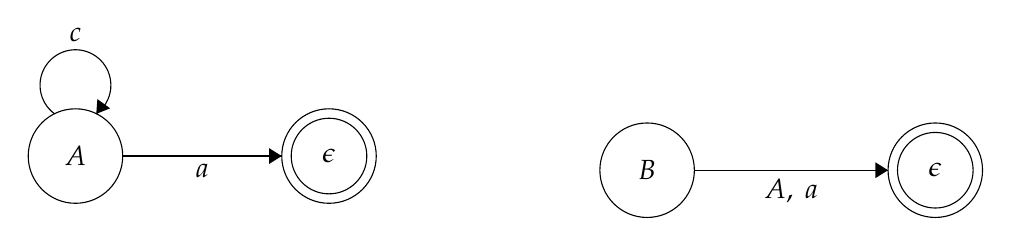
\begin{tikzpicture}[scale=0.2]
\tikzstyle{every node}+=[inner sep=0pt]
\draw [black] (11.2,-14.4) circle (3);
\draw (11.2,-14.4) node {$A$};
\draw [black] (47.5,-15.3) circle (3);
\draw (47.5,-15.3) node {$B$};
\draw [black] (65.8,-15.3) circle (3);
\draw (65.8,-15.3) node {$\epsilon$};
\draw [black] (65.8,-15.3) circle (2.4);
\draw [black] (27.3,-14.4) circle (3);
\draw (27.3,-14.4) node {$\epsilon$};
\draw [black] (27.3,-14.4) circle (2.4);
\draw [black] (9.877,-11.72) arc (234:-54:2.25);
\draw (11.2,-7.15) node [above] {$c$};
\fill [black] (12.52,-11.72) -- (13.4,-11.37) -- (12.59,-10.78);
\draw [black] (14.2,-14.4) -- (24.3,-14.4);
\fill [black] (24.3,-14.4) -- (23.5,-13.9) -- (23.5,-14.9);
\draw (19.25,-14.9) node [below] {$a$};
\draw [black] (50.5,-15.3) -- (62.8,-15.3);
\fill [black] (62.8,-15.3) -- (62,-14.8) -- (62,-15.8);
\draw (56.65,-15.8) node [below] {$A,\mbox{ }a$};
\end{tikzpicture}
\end{center}		
\decoRule
\caption[Conflicts in a graph]{Machine B has a conflict on encountering a terminal 'a'}
\label{fig:ConflictExample}
\end{figure}

	\pagebreak
	\subsubsection{Example}
	As the original example grammar did not contain any conflicts, the figure above will be used as an example. It shows two machines, one for the non-terminal $A$, and one for the non-terminal $B$. Now, for the output of the algorithms and functions below:\\
	\begin{align*}
	&alphabetOfState(A, M(A)) = \{a,\ c\}\\
	&alphabetOfState(\epsilon, M(A)) = \{\}\\
	&alphabetOfState(B, M(B)) = \{a,\ A\}\\
	&alphabetOfState(\epsilon, M(B)) = \{\}\\\\
	&firstTerminalOf(M(A), \{A, B\}, \{M(A), M(B)\}) = \{a, c\}\\
	&firstTerminalOf(M(B), \{A, B\}, \{M(A), M(B)\}) = \{a,\ c\ (from\ M(A))\, a\ (from\ M(A))\}\\\\
	&findConflicts(M(B), \{A, B\}, \{M(A), M(B)\}) = \{(B, A, \epsilon)\}\\
	&\qquad 1\ conflict\ in\ M(B)\ being:\ from\ B,\ taking\ A,\ to\ \epsilon\\
	&findConflicts(M(A), \{A, B\}, \{M(A), M(B)\}) = \{\}\\
	&\qquad 0\ conflicts\ in\ M(A)\\
	\end{align*}
	Below are the resulting machines shown that come from the algorithm. Left is the NFA obtained from only replacing the transition with the entire machine. Right is the DFA that is obtained from this NFA. With that, the DFA is the output of \textit{solveConflicts($M(B), \{M(B), M(A)\}, \{A, B\}, \{(B, A, \epsilon)\}$}).
	\begin{figure}[H]
		\centering
		\includegraphics[width=\textwidth, keepaspectratio]{Figures/conflictSolvingChap2.png}
		\decoRule
	 	\caption[Conflict resolving NFA to DFA]{The NFA obtained from replacing the conflicting transition and the DFA obtained from the NFA.}
	 	\label{fig:chap2:NFA2DFA:ConflictSolving}
	\end{figure}
	
	
	\pagebreak
	\begin{algorithm}
	\caption{Resolve Conflicts}	\label{alg:conflicts}
	\begin{algorithmic}[1]
		\Function{solveConflicts}{dfa, allDfas, nonTerminals, conflicts}
		\ForAll {$\{tr | tr \in conflicts\}$}
			\State $nfa \gets replaceTransitionWithMachine(tr, dfa)$
		\EndFor
		\State $dfa \gets NFA2DFA(nfa)$
		\State $newConflicts \gets findConflicts(dfa, nonTerminals, allDfas)$
		\If {$newConflicts \not = \{\}$}
			\State \Return $solveConfcicts(dfa, allDfas, nonTerminals, newConflicts)$
		\Else	
			\State \Return $dfa$
		\EndIf
		\EndFunction
	\end{algorithmic}
\end{algorithm}
\vfill
\begin{algorithm}
	\caption{Find Conflicts}
	\begin{algorithmic}[1]		
		\Function{findConflicts}{dfa, nonTerminals, allDfas}
			\State $conflicts \gets \{\}$
			\ForAll {$\{state | state \in dfa.Q\}$}
				\State $tokens \gets alphabetOfState(state, dfa)$
				\State $ntsOfState \gets \{nt | nt \in tokens \land nt \in nonTerminals\}$
				\State $terminalsOfState \gets tokens - ntsOfState$
				\ForAll {$\{nt | nt \in ntsOfState\}$}
					\State $nextTerminals \gets firstTerminalOf(allDfas[nt], nonTerminals, allDfas)$
					\If {$(nextTerminals - terminalsOfState \not = \{\})$}
						\State $conflicts \gets conflicts + (state, nt, dfa.\delta(state, nt))$ 
					\EndIf
				\EndFor
			\EndFor
		\State \Return $conflicts$
		\EndFunction		
	\end{algorithmic}
\end{algorithm}
\vfill
\begin{algorithm}
	\caption{Get the terminals reachable from the first state of a machine}
	\begin{algorithmic}[1]		
		\Function{firstTerminalOf}{dfa, nonTerminals, allDfas}
			\State $tokens \gets alphabetOfState(dfa.q_0, dfa)$
			\State $terms \gets tokens - nonTerminals$
			\State $result \gets terms$
			\ForAll{$\{nt | nt \in (tokens - terms)\} $}
				\State $result \gets result + firstTerminalOf(allDfas[nt], nonTerminals, allDfas)$
			\EndFor		
			\State \Return $result$
		\EndFunction
	\end{algorithmic}
\end{algorithm}
	\pagebreak
	
	\subsection{Mapping machines to contexts}
	Once all non-terminals have their own conflictless machine it is possible to make a deterministic mapping from the machines to contexts and respective scopes. The general idea is to define a datatype corresponding to a state-based syntax highlighter. An algebraic datatype works very well because of the nested structures of a highlighter. Once the machines are translated into this datatype, define different methods on this datatype in order to write out highlighters for different editors. One general $SyntaxHighlighter$-datatype like this greatly improves on extensibility to new editors that use a similar structure. An alternative approach could be to define one $SyntaxHighlighter$-datatype per editor and write a specific machines-to-highlighter function per editor.\\\\
	The first of the aforementioned approaches is chosen and this translation step from machine to highlighter can be described as follows:
	\begin{enumerate}
	\item For each machine $M$ create a context $c_q$ per state $q \in M.Q$
	\item For each context $c_{q_1}$ add matches for each $tr=(q_1,\ a,\ q_2) \Rightarrow q_1, q_2 \in Q \land a \in \Sigma$:
		\subitem $c_{q_1}.matches$ += $(a,\ null(),\ set(c_{q_2}))$
	\item For context $c_{q_1}$ add matches for each $tr=(q_1, A, q_2) \Rightarrow q_1, q_2 \in Q \land A \in V$:
		\subitem $tokens = firstTerminalsOf(M(A))$
		\subitem $c_{q_1}.matches$ += $(lookahead(any(tokens)),\ null(),\ set([c_{q_2},\ c_{A.q_0}]))$\vspace{0.05in}\\
		The regular expression is supposed to be a lookahead match on any of the terminals of the machine $M(A)$. This is needed because lookahead does not consume the actual pattern that was matched. This will be done by the first context of $M(A)$. The action replaces the old context $c_{q_1}$ with the $c_{q_2}$ and pushes the first context of machine $M(A)$ called $c_{A.{q_0}}$ on top of that. So the highlighter is now in machine $M(A)$ and once this pops itself off, it ends up in the next state of the original machine. 
	\item For each context $c_{A.q} \Rightarrow q \in M(A).F$ take one of the action described in the next section (\nameref{sec:FinalStateCases}).
	\item For the start symbol $S$ create a context $c_{main} = include(c_{S.{q_0}})$
		\subitem Creates an empty $main$ context that includes the first actual context.
		\subitem $H.main = c_{main}$
	\item Identify all matches that need to have a scope assigned and do so. This can be done based on the information gathered in \ref{sec:Pipeline}. For giving entire machines a scope you need to assign the scope to all matches of all contexts corresponding with this machine.
	\item Remove all contexts that are unreachable
	\end{enumerate}
	
	\pagebreak
	
	\subsubsection{Final State Cases} \label{sec:FinalStateCases}	
	There are two cases for a final state of a machine. The state is either final with no outgoing arcs (I.E. a \textit{sink-state}). Or it still has other outgoing arcs (\textit{non-sink state}). These cases could be treated differently when mapping them to contexts.
	\begin{itemize}
		\item \emph{\textbf{Sink-states:}}\\
		For each sink-state there will be no match created (yet), because it has no outgoing arcs. The only thing to be added is a match that pops this context and machine off of the stack.\\
		Let a final sink-state be $q_{fs}$ then:
			\subitem $c_{q_{fs}}.matches$ += $(\epsilon,\ null(),\ pop())$\vspace{0.05in}\\
			This just matches the empty regex, this always succeeds, and then pops. A different approach would be to choose, in the last match that would lead to $c_{q_{fs}}$, to $pop()$ here and to not $push()$ nor $set()$ this context in the first place. In terms of the above sketch:
			\subitem For each $c_{q_1} \in C$, for each $tr:(q_1,\ a,\ q_{fs}) \Rightarrow q_1, q_{fs} \in Q \land a \in \Sigma$
				\subsubitem $\quad c_{q_1}.matches$ += $(a,\ null(),\ pop())$
			\subitem For each $c_{q_1} \in C$, for each $tr:(q_1, A, q_2) \Rightarrow q_1, q_{fs} \in Q \land A \in V$
				\subsubitem $\quad tokens = firstTerminalsOf(M(A))$
				\subsubitem $\quad c_{q_1}.matches$ += $(lookahead(any(tokens)),\ null(),\ set(c_{A.q_0}))$
		\item \emph{\textbf{Non-Sink states:}}\\
		These states are harder to reason about. There are choices that need to be made, which is hard to do in a deterministic way. A state like this means that you can either \emph{pop} the current machine, or continue consuming with this machine. There could be conflicts here again as well, for example:
		\subitem The current machine is $B$.
		\subitem A final non-sink state $A.q_f \in F$ has 1 transition: $tr=(q_f,\ a,\ q_f)\ :\ a \in A.\Sigma$
		\subitem The state $B.q_x$ has a transition: $tr=(q_x,\ a,\ q_y)\ :\ a \in B.\Sigma$			
		\subitem The context stack looks like this: $[c_{B.q_x},\ c_{A.q_f}]$
		\subitem This is a conflict, do you pop and consume $a$, or continue and consume $a$?
		\subitem There is a choice to be made:
			\subsubitem 1. Resolve these end-of-machine conflicts
			\subsubitem 2. Always pick the $pop$-action
			\subsubitem 3. Always pick the $continue$-action
		\subitem Highlighters do not need to be perfect, so for now pick option 3.
		\subitem To accomplish this, add the same match as if this were a \textit{sink-state}.
		\subitem This has to be the final match, or the other matches become unreachable.
	\end{itemize}
	\pagebreak
	
	\subsubsection{Example}
	Below is a stepwise example of the just described mapping of the machine shown in figure \ref{fig:chap2:NFA:Statement}. For ease of reading it is written in Sublime Syntax format.
\begin{enumerate}
\item For each machine $M$ create a context $c_q$ per state $q \in M.Q$
\begin{lstlisting}[language=SublimeSyntax]
Statement_St:
Statement_0:
Statement_1:
Statement_2:
Statement_3:
Statement_4:
Statement_5:
Statement_6:
Statement_epsilon:
\end{lstlisting}
\item For each context $c_{q_1}$ add matches for each $tr=(q_1,\ a,\ q_2) \Rightarrow q_1, q_2 \in Q \land a \in \Sigma$:
\begin{lstlisting}[language=SublimeSyntax]
Statement_St:
	- match: 'if'
	  set: [Statement_3]
Statement_0:
	- match: ':='
	  set: [Statement_1]
Statement_1:
Statement_2:
Statement_3:
	- match: '('
	  set: [Statement_4]
Statement_4:
Statement_5:
	- match: ')'
	  set: [Statement_6]
Statement_6:
	- match: '{'
	  set: [Statement_St]
Statement_epsilon:
\end{lstlisting}	
\item For context $c_{q_1}$ add matches for each $tr=(q_1, A, q_2) \Rightarrow q_1, q_2 \in Q \land A \in V$:
\begin{lstlisting}[language=SublimeSyntax]
Statement_Start:
	- match: 'if'
	  set: [Statement_3]
 	- match: '?=([a-z]+)'
	  set: [Statement_0, Id_Start]
Statement_0:
	- match: ':='
	  set: [Statement_1]
Statement_1:
 	- match: '?=(\"|[0-9]+)'
	  set: [Statement_2, Literal_Start]
	  
Statement_2:
 	- match: '?=((}| ))'
	  set: [Statement_epsilon, Statement_end_Start]
Statement_3:
	- match: '('
	  set: [Statement_4]
Statement_4:
 	- match: '?=([a-z]+)'
	  set: [Statement_5, Condition_Start]
Statement_5:
	- match: ')'
	  set: [Statement_6]
Statement_6:
	- match: '{'
	  set: [Statement_Start]
Statement_epsilon:
\end{lstlisting}
\item For each context $c_{A.q} \Rightarrow q \in M(A).F$ take one of the action described in \nameref{sec:FinalStateCases}.
\begin{lstlisting}[language=SublimeSyntax]
Statement_epsilon:
	- match: ''
	  pop: true
\end{lstlisting}
\item For the start symbol $S$ create a context $c_{main} = include(c_{S.{q_0}})$
\begin{lstlisting}[language=SublimeSyntax]
main:
	- include: Statement_Start
\end{lstlisting}
\item Identify all matches that need to have a scope assigned and do so. This can be done based on the information gathered in \ref{sec:Pipeline}. For giving entire machines a scope you need to assign the scope to all matches of all contexts corresponding with this machine.
\begin{lstlisting}[language=SublimeSyntax]
Statement_Start:
	- match: 'if'
	  scope: keyword.control.flow
	  set: [Statement_3]
 	- match: '?=([a-z]+)'
	  set: [Statement_0, Id_Start]
\end{lstlisting}
\item Remove all contexts that are unreachable\\
-
\end{enumerate}
		
% Chapter Template

\chapter{Rascal Implementation} % Main chapter title

\label{chap:Implementation} % Change X to a consecutive number; for referencing this chapter elsewhere, use \ref{ChapterX}

\section{Motivation for Rascal} \label{sec:RascalMotivation}
Rascal is a language workbench. It is also a language to be used for many high-level tasks involving the development of new languages and analysis on those and other languages. Since it is very high-level it makes it easier to tackle a rather difficult problem as this project is faced with. Doing something like this in a language like C would be near-impossible. Rascal provides a grammar formalism, algebraic datatypes and high-level operations on structures like graphs and sets.\\ 
The official website\footnote{source: \cite{website:Rascal}} states:
\begin{quotation}\textit{
"Rascal integrates source code analysis, transformation, and generation of primitives on the language level. It can be used for any kind of metaprogramming task: to construct parsers for programming languages, to analyze and transform source code, or to define new DSLs with full IDE support\ldots\\ Rascal primitives include immutable data, context-free grammars and algebraic data-types, relations, relational calculus operators, advanced pattern matching, generic type-safe traversal, comprehensions, concrete syntax for objects, lexically scoped backtracking, and string templates for code generation."
}\end{quotation}
The feature that is being developed by this project is not yet implemented in Rascal, as Rascal does syntax highlighting based on the $CFG$ inside the Eclipse IDE. Rascal itself is also not exported to the various editors with any proper highlighting. This together with all of the above are reasons why Rascal was chosen as the language to work with for this project.

\pagebreak
\section{Grammar formalism} \label{sec:RascalGrammar}
Rascal\footnote{source: \cite{website:RascalSyntax}} has a build in grammar formalism that can be used to develop grammars. Rascal will then generate a parser for this language and generate parse trees and abstract syntax trees for the grammar. One of the special things about Rascal is that it does not care about the complexity of the grammar. It does not need a grammar that is $LR(1)$, theoretically it can generate parsers for any $CFG$. However, there is often ambiguity found in a grammar, this can cause the parser-generator to fail. For this reason Rascal has something called disambiguation constructs. These are handles for the generator such that it can generate parsers without ambiguity. Since this algorithm operates on the grammar-level there is no need to dive into the parsing and evaluation that Rascal does. It is only important that all features that the grammar formalism uses are covered by the syntax-highlighter generator.

\subsection{Simple grammar definition}
Below is a simple grammar shown in Rascal. The keyword \gram{start} denotes the start-symbol $S$ of a grammar. There are four keywords that denote a non-terminal token. These are \gram{syntax, lexical, layout} and \gram{keyword}. These all have different meanings to the parser-generator. \gram{syntax}-tokens and their rules are internally interleaved with the \gram{layout}-token that is defined for the module the grammar is defined in (or if unspecified the $\$default\$$ layout which is empty):
\begin{center}
\gram{syntax S} \gram{= A B} 
\\internally becomes
\\\gram{syntax S} \gram{= A Layout B}
\end{center} 
\gram{lexical}-tokens are the same as \gram{syntax}, except for the fact that these do not get interleaved with \gram{layout}-tokens. The \gram{keyword}-tokens are a special kind of tokens that are used for disambiguation. It is used for making sure that keywords are not seen as identifiers for example. These tokens can only have single character classes or string literals as their rules. So no non-terminals nor regular expressions.
\lstinputlisting[language=RascalGrammar, caption={A Simple Example Grammar in Rascal}]{Code/grammars/simple/simple.grammar}

\pagebreak
\subsection{More advanced constructs}
	\subsubsection{Regular tokens}
	Rascal has a number of things which help the grammar-writer to develop new grammars quicker without the need to introduce new intermediate tokens to achieve the same result. These are explained and shown below.
		\begin{itemize}
			\item \emph{Character classes}\\
			The simple regular expression concept that defines a character class between square brackets. Negative classes are an option and Rascal supports everything including Unicode characters. Characters are internally represented as integer numbers.
\begin{lstlisting}[language=RascalGrammar]
lexical charclass 
	= [a-z]
	| ![%]
	;
\end{lstlisting}
			\item \emph{Star, Opt and Plus-operator}\\
			The familiar Kleene star and plus operation for zero or more and one or more repetitions respectively. Together with the question mark for zero or one occurrence.
\begin{lstlisting}[language=RascalGrammar]
lexical B_STAR = B*;
lexical B_PLUS = B+;
lexical B_OPT = B?;
\end{lstlisting}
			\item \emph{Begin- and End-of-Line}\\
			Also simple and familiar, the beginning and end-of-line requirements for a regular expression. Denoted with \gram{^} and \gram{\$}.
			\item \emph{Iterseps}\\
			A more special kind of token, also defined on Kleene star and plus with 0 or 1 or more. This is a structure that takes a main token and separator. This means that any list of the \gram{Main} tokens, interleaved with the list of separators, is accepted. This is very handy in for example parsing lists of parameters that are split by a comma.
\begin{lstlisting}[language=RascalGrammar]
lexical ParamList = {IdType ","}*;
/*parses for example: int a, float b, string c*/
\end{lstlisting}
		\end{itemize}
	\subsubsection{Labels}
	Labels are simple structures that allow naming of tokens inside a production rule, or to an entire production rule. Below are \gram{lhs, op, rhs} all labels given to tokens and is \gram{num} the name given to the entire rule with \gram{"42"}.
	\begin{lstlisting}[language=RascalGrammar]
	lexical Exp
		= Exp lhs "+" op Exp rhs
		| num: "42"
		;\end{lstlisting}
		
	\subsubsection{Tags}
	Tags are a special kind of annotation that can be added to production rules. They can give certain messages to the parser-generator. This can be messages like: this type of rule is a comment. Another message not intended for the generator could be: the tokens of this rule should receive a certain colouring. 
\begin{lstlisting}[language=RascalGrammar]
lexical Comment
	= @@Comment>@ "/*" ComChar "*/"
	;
	
lexical String
	= @@Context="string.quoted.doulbe null null null string.quoted.doulbe">@
	  StringBody "\<" Interpolated "\>" StringBody
	;\end{lstlisting}	
	\subsubsection{Disambiguation}
	Rascal has a number of handles to remove ambiguity from a grammar. This is useful for parser-generating, however not always for syntax-highlighting. Nevertheless the implementation should take all these factors into account. 
		\begin{itemize}
			\item \emph{Keywords}\\
			The first is the keywords construct that was mentioned in the previous section. It can be used to match a certain expression minus the tokens specified in a \gram{keyword}. The expression below matches all tokens consisting of the regex, except for those that match something in $Keywords$
			\begin{flushleft}
				\gram{keyword Keywords = "if" \| "else" \| "for" \| "while";}\\
				\gram{lexical Id = [a-zA-Z][a-zA-Z0-9]* \\ Keywords;}
			\end{flushleft}
			\item \emph{Precede and Follow restrictions}\\
			Because Rascal accepts all general $CFG$'s it does not implement longest or shortest match. It matches all possible variants. The only way to force rascal to take either longest and/or shortest match is through follow and precede-restrictions. In simple terms: \gram{[a-z]*} and input \gram{abc}, matches: $[\epsilon, a, b, c, ab, bc, abc]$. One can either enforce that something follows or precedes, but also the 'not' of those two.
			\begin{flushleft}
				\gram{input = 'abc'}
				\\\gram{lexical Id = [a-z]*;}						\hfill 	matches: $\{\epsilon, a, b, c, ab, bc, abc\}$
				\\\gram{lexical Id = [a-z]* !>> [a-z];} 			\hfill 	matches: $\{abc, bc, c\}$
				\\\gram{lexical Id = [a-z] !<< [a-z]*;} 			\hfill 	matches: $\{a, ab, abc\}$
				\\\gram{lexical Id = [a-z] !<< [a-z]* !>> [a-z];} 	\hfill 	matches: $\{abc\}$
			\end{flushleft}
			\item \emph{Associativity}\\
			Rules can receive associativity which reduces ambiguity in parsing. Think of a grammar like expression. Normally you have to write the grammar in a \gram{Exp = Expr "+" Term} way. Otherwise your parse-tree ends up being wrong on evaluation. However Rascal allows \gram{Exp = Exp "+" Exp}, together with the associativity ruling to influence a parse tree to nest correctly and prevent ambiguity. The website states:
\begin{flushleft}\textit{
Using Associativity declarations we may disambiguate binary recursive operators. The semantics are that an associativity modifier will instruct the parser to disallow certain productions to nest at particular argument positions:
\\\indent - Left and assoc will disallow productions to directly nest in their right-most position.
\\\indent - Right will disallow productions to directly nest in their left-most position.
\\\indent - Non-assoc will disallow productions to directly nest in either their left-most or their right-most position.
}\end{flushleft}
			\item \emph{Priority}\\
			Rules can receive priority over other rule(s) which reduces ambiguity in parsing. Think of a grammar like expression. Normally you have to write the grammar in terms of \gram{Exp, Term, Factor} way. Otherwise there is no way to express operator precedence. However in Rascal you can do the following: \gram{Exp = Exp "+" Exp, Exp = Exp "*" Exp}, together with the precedence rules you can parse and find correct parse trees. In the example below, the rule \gram{"42"} has precedence over the "times" operator and that has precedence over the plus.
\begin{lstlisting}[language=RascalGrammar]
lexical Exp
	= "42"
	> left Exp "*" Exp
	> left Exp "+" Exp
	;\end{lstlisting}		
	
	\item \emph{Except}\\
	Except rules are used in order to prevent certain labeled tokens or productions to be matched in a rule. This is done through putting an exclamation mark together with the to-be-excepted labelname at the end of a production rule.
	\begin{lstlisting}[language=RascalGrammar]
syntax S = String!illegal;

lexical String 
	= legal: "whatstringscanbe"
	| illegal: "whatstringscannotbe"
	;\end{lstlisting}
\end{itemize}

\subsubsection{An advanced example grammar}
In appendix \ref{app:Grammars} a grammar is shown that makes use of most of the more advanced constructs that were discussed in these past sections.

\pagebreak


\subsection{Internal representation}
Internally the grammars are represented a little differently. In short, all tokens (terminals and non-terminals), are of a datatype called Symbol. This is an algebraic datatype that can have symbols nested. A production rule also has a datatype called Production. This is also an algebraic datatype that shows a lot of the structure of the formal definition of a rule $p \in P \Rightarrow \prodgr{A}{w}$.
\subsubsection{Symbols}
Symbols are ADT's and divided into four sections seen below. The first one is the one to denote that some symbol is a start symbol. Line four through seven represent the tokens \gram{syntax, lexical, layout, keyword}. The parameterized versions of \gram{syntax} and \gram{lexical} are special versions of these definitions. They can be defined with a special datatype in order to generalize certain symbols. These are virtually nowhere to be found in any grammar used for this project and therefore not much attention was paid to these two symbols.\\ 
Following these lines there are three options defining terminal tokens. These are string-literals, case-insensitive literals and the character-classes.\\
Lines 15 through 22 represent the regular options for a token. Examples of these in order are: \gram{"", A?, A+, A*, \{A ","\}+, \{A ","\}*, (A\|B), (A B)}. These last two are used for alternatives and sequences that are inside a single production rule in parentheses.\\
The final line shows how Conditions are represented. These include all disambiguation constructs on Symbol-level and the begin- and end-of-line operators. The datatype of the Condition can be found in appendix \ref{app:RascalCondition}. 
\lstinputlisting{Code/datatypes/Symbol.data}
\subsubsection{Productions}
The production datatype is the type that represents elements of $P$ in a grammar. Below and in the appendices the datatype is shown. However there a number of unused rules when it comes to the algorithm. The \textit{Rascal Tutor} states:
\begin{itemize}
\item A prod is a rule of a grammar, with a defined non-terminal, a list of terminal and/or non-terminal symbols and a possibly empty set of attributes.
\item A regular is a regular expression, i.e. a repeated construct.
\item An error represents a parse error.
\item A skipped represents skipped input during error recovery.
\item priority means ordered choice, where alternatives are tried from left to right;
\item assoc means all alternatives are acceptable, but nested on the declared side;
\item reference means a reference to another production rule which should be substituted there, for extending priority chains and such.
\end{itemize}
From this it is clear to see that \data{error and skipped} are useless. Less obvious is the regular, one might think that this refers to the regular symbols that are possible. This however refers to the built-in Regex-engine that Rascal has and is therefore not part of this. Reference could be used in a grammar, however this was never encountered during any of the grammars that were tried. Recursive priorities are flattened to only a single priority. Every nested group of rules are rebuild to a \data{\\choice()} and put as a single item in the list of choices in the priority object.
\lstinputlisting{Code/datatypes/Production.data}

\pagebreak

\section{Implementing the Algorithm in Rascal} \label{sec:RascalAlgorithm}
The upcoming section discusses the implementation in Rascal. This includes datatypes, functions and algorithms, however no results or examples are shown. All examples generated from the implementation are results and will be discussed in the corresponding chapter.
\subsection{ToPlainGrammar} \label{sec:RascalFeatureToRemove}
The first step is to reduce the input to a plain grammar that was defined in \ref{sec:CFG_def}. Using all that was discussed above there are number of features that Rascal supports that are not of importance to the algorithm and need to be removed or rewritten. These occur at production- as well as symbol-level. A list of features to be removed or redone at the symbol-level include:
\begin{itemize}
\item labels, they will not be used in the highlighter and can be removed
\item tags that do not describe contexts can be removed
\item conditions, some of these are not important to a highlighter.
	\subitem \data{\\at-column(_)} state-based highlighters do not support a check like this.
	\subitem \data{\\except(_)}, labels were removed so this is not useful anymore either.
\item All regular-symbols can be rewritten to terminals, non-terminals and production rules.
	\begin{lstlisting}[language=RascalGrammar]
	A?				-> A_OPT 								= A | ;
	A+				-> A_PLUS 							= A | A A_PLUS;
	A*				-> A_STAR 							=   | A A_STAR;
	(A | B)		-> A_B_ALT 							= A | B;
	(A B)			-> A_B_SEQ 							= A B;
	{A ","}+	-> A_,_ITERSEPS 				= A A_,_ITERSEPSTAIL
						-> A_,_ITERSEPSTAIL 		= "," A A_,_ITERSEPSTAIL | ;
	{A ","}*	-> A_,_ITERSTARSEPS 		= A A_,_ITERSTARSEPSTAIL | ;
						-> A_,_ITERSTARSEPSTAIL = "," A A_,_ITERSEPSTAIL | ;\end{lstlisting}
\end{itemize}
The Sublime syntax-highlighters support character classes as well and therefore it is unnecessary to remove these. The other conditionals can be represented with a special regular expression using lookahead and lookbehind. Also all tokens that have nested symbols being a terminal are not rewritten to new Symbols but kept as regular expressions. So \gram{[a-z]+} is kept as is and does not become. \\ \gram{[a-z]_PLUS = [a-z] [a-z]_PLUS \| [a-z];}\\\\
The best approximation of a formal production rule $p \in P$ is the\\ 
\data{\\prod(Symbol lhs, list[Symbol] rhs, set[Attr] attributes)}.\\
Of the productions that can be encountered there are 3 in conflict: \data{priority},\\ \data{associativity} and \data{choice}. Choice only holds a set of Productions together with the left-hand symbol that these have in common. If all elements of choice are of type \data{prod}, then choice can remain for ease of use. A highlighter does not produce parse-trees so the associativity rules are not important and can therefore be removed. This is done through extracting the set of alternatives from the Production and removing the associativity attributes from the rules found in the set.\\
For priority there are two options. Either rewrite the rules to keep the structure, or just remove them as done with associativity. The first option is like rewriting\\
\gram{Exp = "42" > Exp "*" Exp > Exp "+" Exp;}\\
to\\
\gram{Exp = Exp "+" Exp \| Exp1; Exp1 = Exp1 "*" Exp1 \| Exp2; Exp2 = "42";}\\
The second option is just like with associativity and flatten priority to a choice Production. I have implemented both versions which will be discussed in the \nameref{chap:results} chapter. The nice thing about rewriting it in this way is that you can keep using the grammar formalism of Rascal and all its features, like writing an internal representation back to the human representation.

\subsubsection{Layouts}
I chose to remove all layouts from all of the production rules. This is due to the fact that generally the \gram{layout}-tokens are used for 2 things: whitespace and comments. Although comments are important to the highlighter, whitespace is not. I chose to extract them from the productions but keep them behind such that these can go into a prototype context\footnote{prototype contexts were contexts that are always included (\ref{sec:SublimeSyntax})}. This way the rest of the machines become way less cluttered with possible whitespace parsing.

\subsubsection{Scope information extraction}
The preserving of the scopes to be assigned are handled in the beginning of the process. Every symbol of the simplified grammar is mapped to the corresponding scope that is saved for later use. However there is a limitation in the current implementation which causes loss of power in the potential highlighter. This is the fact that any token can only have one scope assigned to it over the stretch of the entire grammar. This is true for non-terminals as well as terminals (so no different colouring between function call, definition or variable declaration identifiers). If nested conflicts arise then the deepest scope is assigned to the matched token. (E.G. an entire machine of some non-terminal wants scope A and a Token inside this non-terminal's rules has scope B). Due to a lack of time and performance of the algorithm this was implemented in this way and not extended to the better variant described in earlier chapters.

\pagebreak

\subsubsection{The implementation}
The runtime of this part of code is linear with the size of the input grammar, where the size of a grammar is defined by the number of production-rules together with the total number of Symbols present in the grammar (including nested ones). This can be seen in the function below. First it rewrites all rules of a grammar to a set of plain elements of the type \data{\\prod(Symbol lh, list[Symbol] rhs, set[Attr] attributes)}. After this, all symbols in the right-hand side of a rule are rewritten in the way that was just described. Then, as a final action, based on the passed parameter, remove all the interleaved \gram{layout}-tokens. However, rules corresponding to layouts themselves are kept. This results in a new grammar in which by normal means the \gram{layout}-symbols are unreachable, however this is fixed through adding them as a prototype context later.
\lstinputlisting[language=Rascal]{Code/ToPlainGrammar.rsc}


\subsection{Grammar2Graph}
There was already something present in Rascal that created a graph with dependencies of symbols. This however did not search recursively enough, so I wrote my own variant that dives recursively into a symbol and finds any general non-terminal token that is not inside a \data{Condition}. The build-in Graph datatype is nice and generically written, however the function to compute its strongly connected components was not yet implemented. So I implemented Kosaraju's algorithm in order to compute the components.\\\\
Both the \emph{grammar2graph} and \emph{Kosaraju's Algorithm} are shown below. The functioning of \textit{grammar2graph} can be written as: For each \data{Symbol elem} in the right hand side of any rule in the grammar, check whether the left-hand side $s$ is a label with a plain symbol or a plain Symbol itself. Assign the name $from$ to the plain symbol. Now if $from$ is some instance of a non-terminal, enter the second for-loop. For each symbol that is a plain non-terminal token inside $elem$ (including $elem$ itself), add an edge from the symbol $from$ to the plain non-terminal that was found.\\
One extra feature was added to this function. Every vertex gets a self-loop. This is because of Rascal's graph implementation being just the set of edges. This disallows disconnected vertices to be part of a graph. To circumvent this, I added this little line that is not entirely correct, but helps Kosaraju's algorithm to find all components, including singular components with no edges.\pagebreak
\lstinputlisting[language=Rascal]{Code/Grammar2Graph.rsc}

\subsubsection{Kosaraju}
Below is the algorithm of Kosaraju shown. $components$ is a map that maps every edge to its corresponding component. Returning the range of this map is the set of strongly connected components. It is written generically so it can be used on any Rascal-defined Graph.
\lstinputlisting[language=Rascal]{Code/Kosaraju.rsc}

\pagebreak
\subsection{ToStronglyRegularGrammar}
The transformation described in \cite{MohriNederhof} is implemented in rascal. It handles all symbols except parameterized lexicals and parameterized syntax-tokens. These throw exceptions everywhere they cause a problem, so this is easy to extend. These were never encountered so not really in scope for this project. The conversion is preceded by performing the $ToPlainGrammar$-function, since it expects a grammar consisting of only \data{\\prod(_,_,_) and \\choice(_,_)}. As an intended side-effect this transformation removes all attributes from the grammar. This makes the new grammar loose all information on contexts and scopes since this should be extracted from the plain version of the grammar and not the strongly regular one. Below is the \emph{strongly regular} version of the expression-grammar. The $A'$s are replaced with $A\_end$, since the primed versions of the tokens correspond to parsing the ending of a token.

\subsection{Converting the grammar to StateMachines} 
After the grammar is rewritten to a strongly regular one it needs to be rewritten to a set of statemachines. Rascal has a datastructure callled \data{map[&T from, &S to]}. This can be used to map a single Symbol or set of Symbols (I.E. a component) to a StateMachine. Using the algorithm from \ref{sec:ComponentMachine} the machines can first be generated per component and then mapped to the Symbols which are then mapped to $DFA$'s. This is done through the standard powerset construction. So no NFA's per component because the next step is to convert them to DFA's. The implementation is slightly different from the one described, because it introduces a few extra states. Instead of introducing one transition $(q_S,\ a,\ q_B)$ for the rule \data{S = "a" B}, there are two rules introduced: $(q_S,\ a,\ q_{term\_a})$ and $(q_{term\_a},\ \epsilon,\ q_B)$. These intermediate states are all uniquely named. Therefore, not every instance of a terminal $a$ goes to the, same $q_{term\_a}$.

\pagebreak
\subsubsection{StateMachine datatype} \label{sec:RascalStatemachine}
In the section below\footnote{In the actual code $delta$, $q0$ and $F$ are replaced with $transitions$, $startState$ and $finalStates$.} the datatype of a StateMachine is shown. States are represented by strings, a Token is something that can be on an arc, which in this case is a Symbol. A Transition is a 3-element tuple that holds two states, from and where, and a Token that triggers the transition. A DeltaFunction is a set of Transitions that can be indexed as an array. For example: Transition tr[$s_0$] returns a set of 2-element tuples of type \data{set[tuple[Token, State]]}, which are all possible combinations of tokens and resulting state that $s_0$ has in the machine. Now a statemachine is either an $NFA$ or a $DFA$. This is decided with the constructor that is chosen on instantiation. There is no actual prevention of adding non-determinism to a $DFA$. This is left to the programmer. For $\epsilon$-transitions I created an extension to Rascal's Symbol called \data{\\eps()}. As can be observed the states are not saved as separate items in the machine since they can be obtained from $\delta$.
\lstinputlisting[basicstyle=\ttfamily\small]{Code/datatypes/StateMachine.data}

\subsubsection{Conflict resolution} \label{sec:RascalConflicts}
Resolving the conflicts is done as described in \ref{sec:ConflictResolutionAlgorithm}. This is done is almost the exact way the algorithms describe. 

\subsection{Mapping to Contexts} \label{sec:RascalToContexts}
The mapping to contexts is largely done through the description in chapter \ref{chap:Algorithm}. Rascal has a few extra features that are left to consider, being the Conditional Symbols. These are harder to process since the conditions themselves can result in a prefix or a postfix of a regular expression. For example: \gram{[a-z] !<< [a-z]+ !>> [a-z]} can be expressed with lookahead and -behind as \data{(?<![a-z])([a-z]+)(?![a-z])}. Luckily they are all expressable in the regex engine that Sublime and other editors like TextMate use. Precede and follow restrictions translate into lookbehind and lookahead. The \data{\\delete(_)} becomes negative lokahead before the actual match (E.G. \data{id \ "for"} result in match: \data{'(?!for)(id)'}). The begin and end-of-line are also implemented in the regex engines as the same tokens. So except for doing a few tricks with generating correct regular expressions this step is done in the same manner as was described in the previous chapter.

\pagebreak
\subsubsection{Highlighter datatype} \label{sec:RascalHighlighter}
Below is the datatype that represents a state-based syntax highlighter in Rascal. It represents much of the structure of a Sublime Highlighter, but with minimal extensions or modifications other editors could be added. There is also a function that writes an instance of this type to a \emph{.sublime-syntax} file. An $SHRegex$ is regular expression to be set as a match. The SyntaxHighlighter is the top level object. It contains a set of $SHVar$ which are named regular expressions that can be defined for reuse. The rest of the constructors and types speak for themselves.
\lstinputlisting{Code/datatypes/Highlighter.data}
\chapter{Results \& Evaluation} % Main chapter title

\label{chap:results} % Change X to a consecutive number; for referencing this chapter elsewhere, use \ref{ChapterX}

%\Large WRITE A LITTLE BIT ABOUT WHICH EXAMPLES ARE SHOWN. 
%\normalsize

In this section I will discuss a number of cases and snippets to showcase the results and behaviour of the implemented algorithm. This includes trade-offs, design choices and flaws. In this section the different reasons that cause problems in the final highlighters will become apparent as well as which parts are very useful for the process.

\section{Embedding scope information}
The system of embedding highlighting information established in \ref{sec:Pipeline} is quite literally used in the Rascal grammars. An example of this is included here as well as in the appendix (\ref{app:advancedGrammar:contexts}). A number of things become clear about this way of embedding information:
\begin{itemize}
\item[]\emph{Pros:}
\subitem 1. Assigning scopes in this manner is easy and intuitive. 
\item[]\emph{Cons:}
\subitem 1. Having to write the entire scope for every rule quickly becomes tedious. 
\subsubitem Especially for simple cases (E.G. \gram{MyKeywords}). 
\subitem 2. Unable to assign scopes to nested symbols that rascal views as one. 
\subsubitem For example: \gram{"+" and "-"} inside the last priority group of \gram{Expression} 
\subitem 3. Knowledge of what Rascal sees as one symbol and what not is required.
\subsubitem \gram{Identifier} has only 1 symbol on its right-hand side.
\end{itemize}
\pagebreak
\lstinputlisting[language=RascalGrammar, caption={The advanced example grammar with scope information}]{Code/grammars/RascalExp/RascalEx_withContexts.grammar} 
To make the process of scope assigning less tedious, one could add scopes on Symbol level as well as production level. In this way \gram{MyKeywords} could get one scope assigned instead of four times the same one. To circumvent the second issue, one has to rewrite parts of the grammar that are in specific need of colouring. This is not the end of the world, but not preferable. A better possible approach would be to allow the assigning of scopes to labels. Since labels can be found and assigned inside the nested symbols of a production. The third issue is not as much an issue in the sense that it obstructs the usefulness of the algorithm, however it represents the fact that the implementation is not very user-friendly towards beginners of Rascal.

\section{Simplifying the grammar}
Inside the project there is a module called \emph{ToPlainGrammar}. This module does the rewriting of a standard Rascal grammar to the plain form. Results of this can be viewed below. This is done in smaller snippets from larger grammars. 2 snippets are shown here, the Expression non-terminal of the grammar in the previous section. The second snippet shows a formulation for a list of declarations.\\
For a complete look at the pipeline one can look at appendix \ref{app:advancedGrammar} through \ref{app:pico}. There are two forms of the \textit{toPlainGrammar}-function, one that preserves the priority and one that does not. The first can be viewed in the appendices, the second is used here.

\pagebreak
\lstinputlisting[language=RascalGrammar, caption={Snippets showcasing the behaviour of \textit{ToPlainGrammar}}]{Code/grammars/results_simple.grammar}
As seen above the removal of unwanted features functions as it should. It properly rewrites regular structures into a set of non-terminals, terminals and productions. It also properly removes parse-tree altering structures on the rules as well as labels and some of the tags (last of these are removed in the \textit{ToStronglyRegular}-section). The original version did not account for \gram{layout}-symbols nor for parameterized tokens. These are all taken care of in this new implementation as well.

\subsection{Scope information}
The scope-information that is present in the grammar is saved in a proper manner. The contexts are saved as tags which are of type \data{Attr}. These end up being in the \data{\\prod(_,_,set[Attr] attributes)}. Therefore rewriting the rules to \data{\\prod(_,_,_) or \\choice(_,_)} does not cause any loss of information. The symbol rewriting does not cause loss of information, because everything that is seen by the parser as one token is rewritten to still be one token (E.G. \gram{syntax A = A (B C) \{D ","\}+ ;} has only 3 tokens). These are kept during this transformation and will be extracted from the "plain grammar" once requested by the algorithm.

\section{ToStronglyRegularGrammar}

\subsection{Grammar2Graph}
The method present that converted a grammar into a graph did not perform well enough and has been rewritten to recurse (deeper) into tokens in order to find the deepest symbols present. The function visits all right-hand side elements once. Therefore this conversion runs in linear time with the size of the total amount of symbols of the grammar (nested included).

\subsection{Kosaraju}
Below the set of components of the advanced example grammar (Rascal expression) as well as the strongly regular version are shown. As can be observed, \gram{keyword MyKeywords} is nowhere to be found. This is due to the fact that keywords are always excluded since they only serve as disambiguation constructs and never as real non-terminals. They could never be rewritten to other non-terminals because of the implementation of the Rascal-language.
\begin{lstlisting}
//Original version
set[set[Symbol]]: {
  {sort("Expression")},
  {layouts("MyLayout")},
  {lex("Identifier")},
}
//Strongly regular version
set[set[Symbol]]: {
  {
    sort("Expression"),
    sort("Expression_end")
  },
  {layouts("MyLayout")},
  {lex("Identifier")}
}
\end{lstlisting}

\pagebreak
\subsection{Mohri and Nederhof's transformation}
In appendix \ref{app:MohriGrammar} the example from the original paper is included together with the output this module produces. It has some meaningless productions, this is part of the algorithm and the rules that it produces. Self-loops of the type $\prodgr{A}{A}$ could be removed.\\
Below the advanced example grammar is shown again, it shows how \data{Expression} is rewritten into two non-terminals being \data{Expression and Expression_end}.
\lstinputlisting[language=RascalGrammar, caption={The strongly regular approximation of the advanced expression grammar (\ref{app:advancedGrammar:stronglyregular})}]{Code/grammars/RascalExp/stronglyRegular.grammar}
The implementation of Mohri and Nederhof's algorithm works for all the cases that were tested and shown in this thesis, however there is an edge-case that is not covered in the implementation. This throws a warning, so once someone meets this edge-case it will be noticed. The case is matched when a mutually recursive set of non-terminals is completely left-linear, but not right-linear. If all rules are left-linear then this set of rules should not be rewritten. However on converting this set of rules to a NFA the algorithm crashes because it uses the simple NFA-construction algorithm from a right-linear grammar. In order to circumvent this one could rewrite the left-linear sets to right-linear ones with the standard rewriting-algorithm. 




\pagebreak
\section{The \emph{Strongly Regular Grammar} to StateMachines} \label{sec:results:strReg2machines}
In the appendix a number of NFAs as well as DFAs are included for other grammars and tokens. Here is a DFA and corresponding grammar that show the results of the algorithm and some of its flaws. 

\lstinputlisting[language=RascalGrammar, caption={A grammar showing nested comments}]{Code/grammars/comments/comments.grammar}
\begin{figure}[h!]
	\centering
	\includegraphics[width=\textwidth, keepaspectratio]{Figures/comment_dfa.png}
	\decoRule
 	\caption[DFA for Comment]{The DFA for Comment, produced from the strongly regular approximation}
\end{figure}
At first the machine seems proper, if one were to feed this a nested comment as input it is clear that it could consume this. This is good because it guarantees that there was no loss in information up till here. In terms of the algorithm and the final results however, this is a point which leads to problems in the final highlighter. When writing highlighters by hand, highlighting nested comments is easy because of the context-stack. The flow is simple: on opening comment push a comment context onto the stack, on closing comment pop a comment context off of the stack. The algorithm is designed in a different way, it creates a machine for each component and only pushes a machine if it finds a non-terminal on an arc such that when the pushed machine pops itself off, we end up in the next state. This ensures that within the machine above only the ComChar machine can be pushed, but never a nested comment machine. The choice made in \ref{sec:FinalStateCases} ensures that we remain in the same machine if we can in a non-sink state (state 3). Since a ComChar generally matches anything, so also code outside a comment, it chooses to remain in the machine forever. On top of that it is able to match as many opening and closing comments as it can without the need for balance. This means that the algorithm loses the possibility to properly highlight nested structures within the same component that require some sort of balancing (like bracket balancing and nested comments).

\section{The conflict resolution}
Implementing this part of the algorithm shows flaws in this step. It does however remove all conflicts in a machine except for the ones mentioned in \ref{sec:FinalStateCases}. These are similar to shift-reduce and reduce-reduce conflicts found in parsers.\\
The issues with this part of the algorithm are: 
\begin{enumerate}
\item This recursive process has a very bad time-complexity. It traverses all symbols in all components and all the transitions in the machines corresponding to these symbols. If a conflict is found, it runs the powerset-construction $NFA2DFA$-algorithm which has a bad time-complexity, and then reruns the search for conflicts.
\item Large grammars generate larger machines. Programming languages build on the recursive structure in a grammar and therefore a number of components tend to be large of size. This leads to enormous NFA's and DFA's. If conflicts arise, which happens at higher level tokens more often (like \gram{Statement} in C), the fixing of these conflicts cause large waiting times. This is due to the bad complexity (see the examples below).\\
Small example: x can be a variable or a function-call. Both have identifiers and are at the start of the statement, this will cause a conflict. 
\begin{lstlisting}[language=C]
void x() { printf("function x\n"); }
int main() {
	int x;
	x = 42;
	x(y);
}
\end{lstlisting}  
\item Another thing adding to the bad runtime of this algorithm is the fact that the machines of different symbols of the same component usually contain (many of) the same conflicts. These are all repetitively found and solved, including nested cases.
\end{enumerate}
\pagebreak
The reason the algorithm does not perform on large grammars is this part of the code. The amount of conflicts there are and that occur in a nested manner increase exponentially. Below is some output that was generated whilst working on the $C$ language in Rascal. It never finishes, but prints some statistics about where it is and what it is doing:

\begin{lstlisting}
	83/123: sort("Specifier__STARSEPS__TAIL_end")
sort("Specifier__STARSEPS__TAIL_end")
working on sort("Specifier__STARSEPS__TAIL_end"), currently with 314 conflicts
pre-nfa2dfa: current number of states: 1072
past nfa2dfa
past finding new conflicts
sort("Specifier__STARSEPS__TAIL_end")
working on sort("Specifier__STARSEPS__TAIL_end"), currently with 206 conflicts
pre-nfa2dfa: current number of states: 163
past nfa2dfa
past finding new conflicts
sort("Specifier__STARSEPS__TAIL_end")
working on sort("Specifier__STARSEPS__TAIL_end"), currently with 360 conflicts
pre-nfa2dfa: current number of states: 2038
past nfa2dfa
past finding new conflicts
\end{lstlisting}
This is the result of around 5 minutes of runtime on one of the tokens  it is handling. This was still a rather simple one because it resolved quickly, however there are 122 other tokens that also need conflict fixing which do not get solved this easily. This clearly shows just how unfeasible this approach is for large grammars. This is 1 machine out of 123 and it ends up with over 2000 states, meaning over 2000 contexts. A second example is a machine for the $Javascript$-grammar. It ran for 10 iterations like above and introduced more conflicts every step than there were resolved. At the 10th iteration it had 3544 conflicts and already 18688 states. After this I cancelled the operation as it took forever.



\section{ToContexts}
In this implementation, replacing an arc in a machine means that this non-terminal on this arc is gone afterwards. If a scope was assigned to this arc that information is lost from that point on, since it becomes part of this machine it will receive custom scopes in the next step of the algorithm. Therefore the highlighting might perform worse than expected. Implementation of this part proved harder since there was a lot of rewriting symbols into regular expressions involved. The information for this process was often not available at this point. Especially handling symbols that were of type \data{conditional(_,_)} proved difficult. There are no real intermediate results from this step as they tie together everything and produce the final highlighters to be discussed in the next section.

\pagebreak

\section{Resulting highlighters}
\subsection{Final results}
Together with an example performance the appendices now show the complete path that a grammar takes through the algorithm together with intermediate results. The results being: original grammar $\rightarrow$ plain grammar $\rightarrow$ strongly regular grammar $\rightarrow$ an example NFA constructed from this regular grammar $\rightarrow$ the corresponding DFA. Finally there is a small example program included in the form of a picture, showing the job the highlighter does. After this I have included the performance of a hand-written highlighter in a picture. The entire highlighters were not included for the very simple reason that they are all very long.\\

\noindent Rascal has a small DSL-like programming language called $Pico$. Pico is a 50 line grammar that generates 566 lines worth of highlighter. Besides the appendices the results of Pico are also included below. 
\begin{figure}[h!]
	\centering
	\includegraphics[width=\textwidth, keepaspectratio]{Figures/highlightShots/pico_generated.png}
	\decoRule
 	\caption[Generated highlighter results for Pico grammar]{Results of the highlighter generated for the pico grammar}
\end{figure}

\pagebreak
\begin{figure}[h!]
	\centering
	\includegraphics[width=\textwidth, keepaspectratio]{Figures/highlightShots/pico_handwritten.png}
	\decoRule
 	\caption[Hand-written highlighter results for Pico grammar]{Results of the highlighter hand-written for the pico grammar}
\end{figure}

\subsection{Pico breakdown}
In this section I will discuss the results as seen above and point out some of the strong parts and flawed parts of the generated highlighter.\\\\
\textbf{The good:}
\begin{itemize}
\item The parser-like behaviour this highlighter shows ensures that accidents like highlighting "else" in a word like "elsewhere" are practically impossible. When writing the hand-written version the 2 in i2d of that output got coloured as a constant, even though the generated version always gets this right.
\end{itemize}
\textbf{The bad:}
\begin{itemize}
\item The "declaration"-section defines 3 variables. These are \data{id}, \data{nat} and\\ \data{noHighlightingOnTheNextLine}. In this section the highlighter expects rules of the type: \gram{Id ":" Type}, where the type should get the scope \data{storage.type}. This works for the first line, however then it encounters an end-of-line, makes the wrong decision to pop because nothing matches. The next line still contains declarations, but receive no highlighting. This is also true for line 13 and 18, because all of 13 is on one line the highlighting is okay, but it fails at 18 again because of new-lines.\pagebreak
\item "if" is not highlighted because it is seen as an identifier by the highlighter. This is because the match for an Id (any combination of letters, so also "if") is tried earlier than the specific match for if.\\
\begin{lstlisting}[language=SublimeSyntax]
  Statement__DQUOTESEMIDQUOTE__STARSEPS_0:
    - meta_scope: Statement__DQUOTESEMIDQUOTE__STARSEPS_0
      # match for id
    - match: '(?=(([\x{61}-\x{7A}])(([\x{30}-\x{39}\x{61}-\x{7A}])*)(?!([\x{30}-\x{39}\x{61}-\x{7A}]))))'
      set: [Statement__DQUOTESEMIDQUOTE__STARSEPS_1, Id_0]
    - match: '(fi)'
      scope: keyword.control.flow
      set: [Statement__DQUOTESEMIDQUOTE__STARSEPS_2]
    - match: '(while)'
      scope: keyword.control.flow
      set: [Statement__DQUOTESEMIDQUOTE__STARSEPS_6]
    - match: '(else)'
      scope: keyword.control.flow
      set: [Statement__DQUOTESEMIDQUOTE__STARSEPS_4]
    - match: '(od)'
      scope: keyword.control.flow
      set: [Statement__DQUOTESEMIDQUOTE__STARSEPS_5]
      # match for not any of the cases (I.E. non-sink state)
    - match: '(?!((while)|(if)|(else)|(od)|(?=(([\x{61}-\x{7A}])(([\x{30}-\x{39}\x{61}-\x{7A}])*)(?!([\x{30}-\x{39}\x{61}-\x{7A}]))))|(fi)))'
      pop: true
    - match: '(if)'
      scope: keyword.control.flow
      set: [Statement__DQUOTESEMIDQUOTE__STARSEPS_3]
\end{lstlisting}
\item The second "\%" on line 15 is not highlighted because the block-comment match is tried before the line comment match. The block-comment expects a \% then anything that is not \% and then a closing \%. It does not highlight the second \% because it is seen as not part of the comment and the line-comment is too far down the context to be tried.
\begin{lstlisting}[language=SublimeSyntax]
  WhitespaceAndComment_0:
    - meta_scope: WhitespaceAndComment_0
    - match: '(%)'
      scope: comment.block
      set: [WhitespaceAndComment_1]
    - match: '([\x{9}-\x{A}\x{D}\x{20}])'
      pop: true
    - match: '(%%)'
      scope: comment.line
      set: [WhitespaceAndComment_2]
\end{lstlisting}
\end{itemize}


\pagebreak
\subsubsection{Statistics on the final results}
Below are a few tables that show and discuss the performance of the highlighters included in the appendices. They are compared with highlighters that were written by hand. In the appendices there are also examples included of the actual highlights the different versions produce.

\begin{table}[h!]
\caption{Statistics on generated highlighters vs hand-written ones}
\label{tab:highlighters}
\begin{center}
\begin{tabular}{|c|c|c|c|c|}
\hline
\tabhead{Name} & \tabhead{Generated} & \tabhead{SLOC} & \tabhead{NumContexts} & \tabhead{Performance (++/+/-/--)} \\
\hline
Nested comments & true & 100 & 11 & --\\
				& false & 27 & 3 & ++\\
\hline
String Interpolation & true & 77 & 11 & ++\\
					 & false & 33 & 4 & ++\\
\hline
Pico & true & 566 & 57 & -\\
	 & false & 61 & 8 & ++\\
\hline
\end{tabular}
\end{center}
\end{table}
\noindent In here it is clear to see that the parser-like behaviour breaks the highlighter. It introduces many lines and contexts that do not contribute to the performance of the highlighters, only in a negative way.


\section{Overall results}
As can be seen in especially the final results, the highlighters do not do a particularly good job. This is mainly due to the following things:
\begin{enumerate}
\item First of all, looking at the nested comment grammar. In converting the strongly regular grammar into machines all elements of a component are put in one machine. In order to properly highlight nested comments a structure like this is needed: On start of new comment $\rightarrow$ push new machine that highlights a comment. On ending of a comment $\rightarrow$ pop the current machine. This is what the stack is useful for, to keep track of how many times the highlighter is nested. However because of the merging of all comments into one machine and the way the $ToContexts$ part is constructed a new machine is only pushed if the highlighter moves from one machine to one that is outside of its current component (I.E. a non-terminal arc). This never occurs for the nested comment case and this is why it accepts endless amounts of opening and closing comments without ever pushing nor popping machines. (\ref{sec:results:strReg2machines})
\pagebreak\item There is also the issue discussed in \ref{sec:SublimeSyntax:LineEndings} that brings problems in the final algorithm. Since the pushing of new machines is triggered on lookahead of one of the starting tokens of that machine, problems arise when end of lines (\$) are the next token to be consumed. The Sublime highlighter matches per-line, so never past an end of line. Let us assume a highlighter has the following context:
\begin{lstlisting}[language=SublimeSyntax]
context1_A:
  - match: '?=(a)'
    set: [context1_B, context2_A]
  - match: '?!(a)'
    pop: true
\end{lstlisting}
If we have input of the type \data{bla bla\|\$a b c} and the highlighter is at |. The highlighter will now check and try the matches of the context in order. The first one fails, because it can't look past a new-line, since it matches one line at a time. Therefore it will arrive at the final match and pop the context off, even though the real next token is $a$ and therefore the highlighter "should" push the next machine on top. This can be seen in the $Pico$ example program as well.
\item A general problem with the approach as a whole is that the algorithm tries to retain as much of the original structure of the grammar as possible. However when looking at hand-written highlighters, those programs do not really care about the grammar, it just searches for words to match and colour them. In other words, the generated highlighters act as parsers. This is bad for a multitude of reasons:
\subitem \textbf{a}. Highlighting will not continue properly once past a syntax error.\\
		(E.G. keyword in a "wrong" place will get no highlighting)
\subitem \textbf{b}. Normal highlighters just skip tokens that do not need highlighting. It simply continues past them. On matching something it colours correspondingly. The parser-like behaviour wants to match every token it encounters otherwise it does not continue to the next context. This is bad for a simple reason: more meaningless matching and trying leads to a larger chance of errors.
\subitem \textbf{c}. It introduces the shift-reduce and reduce-reduce like conflicts found when the highlighter is in the final state of a machine. Even though highlighters should easily be able to highlight grammars outside $LR(1)$. It ensures the need for something like $solveConflicts$, which as been shown to be the reason the algorithm does not perform on large grammars.
\item The last problem is more of a beauty remark. The created highlighters are huge and get out of hand fairly soon. A highlighter that was generated for an 80-line grammar describing JSON objects, generated a highlighter of over 750 lines of code. One can only imagine if this were run on for example the C-language.
\end{enumerate}



% Chapter Template

\chapter{Conclusion} % Main chapter title

\label{chap:conclusion} % Change X to a consecutive number; for referencing this chapter elsewhere, use \ref{ChapterX}

%----------------------------------------------------------------------------------------
%	SECTION 1																			|
%----------------------------------------------------------------------------------------

\section{Answers to subquestions}
In \ref{sec:problemdef:sub} a number of subquestions were posed. These questions are useful in answering the main question of this thesis. The posed questions and their respective answers are:
\begin{enumerate}
	\item[\textit{1.}] How to embed highlighting information in a context-free grammar?
	\\\textbf{\textit{The Algorithm:}}\\
	The idea is to assign scopes (or some other information) to the tokens of production rules. It is intuitive and easy to do, however it might be a good idea to allow certain generalizations, like assigning information to a Symbol as a whole, meaning to all Symbols of all rules at the right-hand side. The embedded information is easy to extract and is relevant for the rest of the algorithm. Changes to the algorithm might enforce the type of information to be changed.
	\\\textbf{\textit{The Implementation:}}\\
	The grammar formalism Rascal uses nicely allows for this kind of embedding. Many types of information, not just scopes, could be embedded with this method. Implementation-wise there were also a number of things that could have been done better. For one, assigning scopes to nested Symbols was impossible. In the \nameref{chap:results} chapter a number of issues and possible solutions were posed. For example assigning to the information to different labels in Rascal would help to circumvent the nested Symbol problem. 
	
	\item[\textit{2.}] Can a Rascal grammar be written as the standard 4-element tuple?\\
	The implementation of $ToPlainGrammar$ shows that this is possible and also generalizes to larger grammars. The algorithm works even on large scale programming languages. It just fails on Rascal itself because of the use of parameterized lexicals and syntax-tokens.
	
	\item[\textit{3.}] How to convert a context-free grammar to a regular grammar approximating the same language?\\
	Mohri and Nederhofs transformation stood for this process. The approximation is correct and still understandable. This is important for the used algorithm, because it converts the grammar to state machines which is not generally possible for context-free grammars.
	
	\item[\textit{4.}] How to create useful state-machines from these approximations?\\
	The state machines generated from the transformed grammars are good for accepting the same language. Again however, this contributes to the parser-like behaviour of the algorithm. They theoretically accept the same language, implementing this is a proper manner introduces errors that are similar to shift-reduce and reduce-reduce conflicts.
	
\pagebreak	\item[\textit{5.}] How to map these machines to an actual state-based syntax highlighter?\\
	The final step is the described mapping algorithm. This works for general cases, but encounters lots of problems for end-of-line characters in Sublime. These cause unintentional popping of contexts, breaking the "parser" that the highlighters try to be. This resulting in bad highlighters. On top of this the machines tend to be quite larger, creating enormous highlighters that are hard to follow by hand and to debug.
\end{enumerate} 

\section{How can we derive state-based highlighters from context-free grammars?}
The question posed at the beginning could be rewritten after this thesis. This thesis has presented a possible approach to this problem and concluded that this is not the correct one. This thesis does not answer the question as a whole, but crosses off the described approach whilst generating lots of new information on the subject.\\
The generated highlighters have trouble navigating past end-of-line characters and act more as parsers than as highlighters. The highlighters perform badly and are for described reasons incapable of highlighting certain recursive structures like nested comments. I think it is still possible to generate highlighters from their definitions, however there is a need for a different algorithm and possibly other embedded information to support this new algorithm.\\\\
I have presented a possible approach to generating state based highlighters from Rascal context-free grammars using a regular approximation algorithm as a starting point. I conclude that, for various reasons, this approach is not capable of creating proper highlighters. Reasons include parser-like behaviour, unintentional popping of contexts on end-of-line characters and incapability of properly highlighting recursive structures. 

% Chapter Template

\chapter{Discussion} % Main chapter title

\label{chap:discussion} % Change X to a consecutive number; for referencing this chapter elsewhere, use \ref{ChapterX}

\section{Strong points}
\subsection{Algorithm}
The algorithm fails to serve its purpose and therefore it has few strong points.The things that are strong about the algorithm is that the way of embedding information is at the right position. It does not ask the grammar-writer to write a separate part additionally to the grammar, but it asks extra information about the grammar. If the corresponding algorithm using this extra information (even if the information would be of a different kind), then generating a highlighter really comes from the grammar and part of the process of creating grammars instead of a separate programming task as a whole.\\
The complexity of the components of the algorithm are also quite good. Usually linear with respect to the size of the input-grammar. Except for the solving of conflicts and the standard $NFA2DFA$ algorithm. This gives hope for other approaches being able to tackle this problem, even for large grammars.

\subsection{Implementation}
The individual parts of the algorithm find use in multiple subjects (Graph theory, language engineering, etc). Therefore implementing all these separate parts were not a waste of time. Rascal did not have functions for computing strongly connected components, nor a highlighter datatype. These and others are examples of things that were created in the process of this algorithm, but reusable for other purposes. A complete list would also include Mohri and Nederhof's algorithm, the statemachine datatype, the $ToPlainGrammar$ functions and the $grammar2graph$-module.\\
Another strong point is the fact that the parts of the highlighters that do work benefit from the parser like behaviour. In handwritten highlighters you often have to delimit matches with word endings (\data{\\b}). These make sure that words like "for" inside therefore do not get highlighted. The generated highlighters do not have this problem since it knows thanks to the context that its parsing something that is not a keyword.

\pagebreak
\section{Weak points}
\subsection{Algorithm}
Due to the nature of state-based syntax highlighters (in at least Sublime) the approach taken will often crash on encountering end-of-lines. This leads to premature popping of contexts and bad highlighting.\\
Secondly, the above error occurs from using lookahead in the highlighter to determine what to do next. This is generally okay, since other highlighters do this as well, however one should be careful in using this. Especially lookbehind and negative lookahead or behind are dangerous to use without an actual match. Since \data{not(something)} is true for lots of cases (E.G. \data{'(?!for)'} returns true for empty string). 
Thirdly, the algorithm to resolve conflicts in the generated statemachines is very inefficient. So bad that for larger grammars the algorithm will take too long to complete. Making it useless on larger grammars.\\\\
Finally, all of the above (and several other) issues with the algorithm would be solved if the algorithm would not induce the parser-like behaviour of the highlighters. Stopping the literal parsing removes lots of the matching and lookahead regular expressions which always results in less possible errors. The generating of machines with all the conflicts is not needed if the highlighter does not care about most of the grammar. These machines will not be generated and therefore no infinite waiting for conflict resolution. If the highlighter simply ignores useless input then also popping on end-of-lines will occur less or not at all.

\subsection{Implementation}
There are also a number of things to be said about the implementation. The realization that the approach would not work came too late and therefore there was no time to retry a different approach. Because of this the code for $ToContexts$ was not written in a proper manner. Long functions and lots of long lines to just get it to work. Time became an issue here and therefore the module $ToContexts$ suffered.\\
Another weak point about the implementation is the way that scopes are saved and then reapplied to the final contexts. As mentioned before the implementation only allows one single context for a single token, wherever it occurs in the grammar. This is not desirable because of described reasons.\\
Finally there is the conflict resolution algorithm substituting the non-terminal tokens on arcs of the machines. If this non-terminal had a scope assigned to it, this information is lost in the process. There should be a better way of keeping track where and to what which information belongs.

\pagebreak
\section{Overall}
The developed algorithm does a poor job at solving the problem, however it generates a sea of information on the topic and nature of the problem. I started off with no knowledge of state-based highlighters and how they work, nor any prior experience in this domain. This makes anticipating future problems very hard. Especially since all the sub-steps seem to work at first, however only in the end it becomes apparent that certain errors slipped in along the way. After this thesis it is clear that this approach does not work and why it does not work. Due to limitations in time there was no time to revert the changes and take a different approach.\\
This thesis and research shows that this approach is not the way to go as it cannot produce proper highlighters for even simple grammars. This is largely due to the parser-like nature of the generated highlighters. I think that fixing this, together with a slightly different way of embedding information could help future researchers a great deal in tackling the same problem once again, but from a different angle. In this new approach much of the created algorithm can be reused in one way or another, paving the path for future solutions to the problem at hand.
% Chapter Template

\chapter{Future \& Related Work} % Main chapter title

\label{chap:futurework} % Change X to a consecutive number; for referencing this chapter elsewhere, use \ref{ChapterX}


\section{Related Work}
Since this project builds on top of many different, relatively easy, concepts there is tons of research already performed on the steps to take for the algorithm. There are a number of things certain.

\subsection{Regular approximations}
The first being that some sort of translation from $CFG$ towards a more regular structure is needed. This is because the state-based highlighters are simple structures that can handle little more than state machines. The algorithm described in \cite{MohriNederhof} proved unsuited for the problem due to the incapability of handling nested structures. This is more due to the translation to state machines than thanks to the described transformation. So some alternatives are needed for which I refer to \cite{evans1997approximating} and \cite{pereira1991finite}.

\subsection{State-based highlighters}
Secondly there needs to be a target highlighter. There is little information on these as every editor uses their own version, however many of them rely on some form of YAML. As a starting point I refer to \cite{website:SublimeSyntax} and \cite{website:TextmateSyntax}.

\pagebreak
\section{Future Work}
In this section I will describe a number of ideas for future research into the research-question. As the problem is not solved I will focus on ideas to solve this problem and less on follow-up research for after this problem.\\\\
The first and foremost problem to be solved is to prevent the parser-like behaviour. There needs to be a more general approach such that the highlighters keep highlighting when syntax errors occur. The simplest approach would be to make a number of contexts that highlight specific cases and to include all of these in the main context. This translates to something like a context for keywords, a (number of) context(s) to highlight strings, same for comments, etc. Then from the main context include all starting-contexts for these concepts. Possible problems for this approach could be that it becomes hard to determine when to nest contexts and how to do this nesting. Think of the example of function-definition identifiers getting a different colour from variable declarations.\\
A second idea could be to embed slightly different information from before. Instead of assigning scopes to the tokens, it might help to let the grammar-writer denote the starting and ending delimiters of a scope. Much like TextMate does in its highlighters. Taking this approach removes the passive popping of contexts because nothing matches, into a more active popping of contexts. Being: If match this, then pop, else stay inside context.\\\\
There is just a general different approach needed to tackle the problem. In future work there might not be a lot of use for the strongly regular grammars either. This is due to the fact that in converting $CFG$s to regular grammars you lose guarantees like bracket balancing. This is something that should never be lost for the problem at hand as state-based highlighters are easily capable of circumventing this problem by using the context-stack. So instead of converting the grammar stepwise to other versions and structures I believe the algorithm should look at the original grammar all the time and try to retrieve the relevant parts from it using this in the generation of a highlighter. So methods for identifying starting and ending delimiters, nested structures and other difficult cases.\\
For the small example in Rascal below this could mean get all keywords and make a context. On opening comment keep colouring everything as a comment until you match the corresponding close. This would result in highlighters that would probably not be as good as a handwritten one, but could do quite a proper job at approximating them without the need for knowledge of the original grammar. 
\begin{lstlisting}[language=RascalGrammar]
keyword Keywords = "for" | "if" | "else" | "while" | "do";
lexical Comment = @@Context="comment.begin null comment.end">@ "/*" ![*] "*/";

\end{lstlisting}

%----------------------------------------------------------------------------------------
%	THESIS CONTENT - APPENDICES
%----------------------------------------------------------------------------------------

\appendix % Cue to tell LaTeX that the following "chapters" are Appendices

% Include the appendices of the thesis as separate files from the Appendices folder
% Uncomment the lines as you write the Appendices

% Appendix Template

\chapter{Grammars} % Main appendix title

\label{app:Grammars} % Change X to a consecutive letter; for referencing this appendix elsewhere, use \ref{AppendixX}

\section{Grammar specifications}

\subsection{Simple example grammar} \label{app:simpleGrammar}
\lstinputlisting[language=RascalGrammar, caption={A simple example grammar}]{Code/grammars/simple/simple.grammar} 

\pagebreak\subsection{Mohri and Nederhof's example} \label{app:MohriGrammar}
\lstinputlisting[language=RascalGrammar, caption={The example grammar that is used in \cite{MohriNederhof} with corresponding outputted grammar from the \emph{ToStronglyRegularGrammar} module}]{Code/grammars/Mohri.grammar}
% Appendix Template

\chapter{Datatypes} % Main appendix title

\label{app:Data} % Change X to a consecutive letter; for referencing this appendix elsewhere, use \ref{AppendixX}

\lstset{language=Rascal}
\lstinputlisting[caption={The Symbol datatype of Rascal}]{Code/datatypes/Symbol.data} \label{app:RascalSymbol}
\lstinputlisting[caption={The Condition datatype of Rascal}]{Code/datatypes/Condition.data} \label{app:RascalCondition}
\lstinputlisting[caption={The Production datatype of Rascal}]{Code/datatypes/Production.data} \label{app:RascalProduction}
\lstinputlisting[caption={The StateMachine datatype in Rascal}, basicstyle=\ttfamily\small]{Code/datatypes/StateMachine.data} \label{app:RascalStateMachine}
\lstinputlisting[caption={The SyntaxHighlighter datatype in Rascal}, basicstyle=\ttfamily\small]{Code/datatypes/Highlighter.data}\label{app:RascalHighlighter}
% Appendix Template

\chapter{Advanced Example Grammar} % Main appendix title

\label{app:advancedGrammar} % Change X to a consecutive letter; for referencing this appendix elsewhere, use \ref{AppendixX}

\subsection{Original definition} \label{app:advancedGrammar:default}
\lstinputlisting[language=RascalGrammar, caption={A grammar that uses almost all constructs. This is a slightly modified version of the one found here: \cite{website:RascalGrammarExample}}]{Code/grammars/RascalExp/RascalEx.grammar}

\subsection{With context information} \label{app:advancedGrammar:contexts}
\lstinputlisting[language=RascalGrammar, caption={The original grammar with contexts}]{Code/grammars/RascalExp/RascalEx_withContexts.grammar} 

\subsection{Simplified without priority} \label{app:advancedGrammar:simple}
\lstinputlisting[language=RascalGrammar, caption={The same grammar but simplified with priority removal}]{Code/grammars/RascalExp/plainGrammar_nopriority.grammar}

\subsection{Simplified with priority} \label{app:advancedGrammar:simplePriority}
\lstinputlisting[language=RascalGrammar, caption={The same simplified grammmar with priority preservation}]{Code/grammars/RascalExp/plainGrammar_priority.grammar}

\subsection{Strongly Regular} \label{app:advancedGrammar:stronglyregular}
\lstinputlisting[language=RascalGrammar, caption={The strongly regular approximation of the original grammar}]{Code/grammars/RascalExp/stronglyRegular.grammar}

\pagebreak\subsection{NFA for strongly regular Expression}
\begin{figure}[h!]
	\centering
	\includegraphics[scale=0.35]{Figures/advancedGrammar_NFA.png}
	\decoRule
 	\caption[NFA for Expression]{The NFA for Expression, produced from the strongly regular approximation}
 	\label{fig:advancedGrammar:NFA:Expression}
\end{figure}


\pagebreak\subsection{DFA for strongly regular Expression}
\begin{figure}[h]
	\centering
	\includegraphics[scale=0.42]{Figures/advancedGrammar_DFA.png}
	\decoRule
 	\caption[DFA for Expresion]{The DFA for Expression, produced from the strongly regular approximation}
 	\label{fig:advancedGrammar:DFA:Expression}
\end{figure}


% Appendix Template

\chapter{Nested Comments Grammar} % Main appendix title

\label{app:comments} % Change X to a consecutive letter; for referencing this appendix elsewhere, use \ref{AppendixX}

\section{Original definition} \label{app:comments:contexts}
\lstinputlisting[language=RascalGrammar, caption={A grammar showing nested comments}]{Code/grammars/comments/comments.grammar}

\section{Simplified without priority} \label{app:comments:simple}
\lstinputlisting[language=RascalGrammar, caption={The same grammar but simplified with priority removal}]{Code/grammars/comments/plain.grammar}

\section{Strongly Regular} \label{app:comments:stronglyregular}
\lstinputlisting[language=RascalGrammar, caption={The strongly regular approximation of the original grammar}]{Code/grammars/comments/StronglyRegular.grammar}

\pagebreak\subsection{NFA for strongly regular Comment}
\begin{figure}[h!]
	\centering
	\includegraphics[width=\textwidth, keepaspectratio]{Figures/comment_nfa.png}
	\decoRule
 	\caption[NFA for Comment]{The NFA for Comment, produced from the strongly regular approximation}
 	\label{fig:comments:NFA:Comment}
\end{figure}

\subsection{DFA for strongly regular Comment}
\begin{figure}[h!]
	\centering
	\includegraphics[width=\textwidth, keepaspectratio]{Figures/comment_dfa.png}
	\decoRule
 	\caption[DFA for Comment]{The DFA for Comment, produced from the strongly regular approximation}
 	\label{fig:comments:DFA:Comment}
\end{figure}

\pagebreak\subsection{Results of generated highlighter}
\begin{figure}[h!]
	\centering
	\includegraphics[width=\textwidth, keepaspectratio]{Figures/highlightShots/comment_generated.png}
	\decoRule
 	\caption[generated highlighter results for NestedComments grammar]{Results of the generated highlighter for this grammar}
 	\label{fig:comments:highlighter:generated}
\end{figure}

\subsection{Results of hand-written highlighter}
\begin{figure}[h!]
	\centering
	\includegraphics[width=\textwidth, keepaspectratio]{Figures/highlightShots/comment_handwritten.png}
	\decoRule
 	\caption[Hand-written highlighter results for NestedComments grammar]{Results of hand-written highlighter for this grammar}
 	\label{fig:comments:highlighter:written}
\end{figure}

% Appendix Template

\chapter{String Interpolation Grammar} % Main appendix title

\label{app:stringInterp} % Change X to a consecutive letter; for referencing this appendix elsewhere, use \ref{AppendixX}

\section{Original definition} \label{app:stringInterp:default}
\lstinputlisting[language=RascalGrammar, caption={A simple string-interpolation language as a Rascal grammar}]{Code/grammars/stringInterp/original.grammar}

\subsection{Simplified without priority} \label{app:stringInterp:simple}
\lstinputlisting[language=RascalGrammar, caption={The plain grammar with priority removal}]{Code/grammars/stringInterp/plain.grammar}

\pagebreak
\subsection{Strongly Regular} \label{app:stringInterp:stronglyregular}
\lstinputlisting[language=RascalGrammar, caption={The strongly regular approximation of the original grammar}]{Code/grammars/stringInterp/stronglyregular.grammar}

\subsection{NFA for strongly regular StringLiteral}
\begin{figure}[h!]
	\centering
	\includegraphics[width=\textwidth, keepaspectratio]{Figures/String_nfa_stringliteral.png}
	\decoRule
 	\caption[NFA for StringLiteral]{The NFA for StringLiteral, produced from the strongly regular approximation}
 	\label{fig:stringInterp:NFA:StringLiteral}
\end{figure}


\subsection{DFA for strongly regular StringLiteral}
\begin{figure}[h]
	\centering
	\includegraphics[width=\textwidth, keepaspectratio]{Figures/String_dfa_stringliteral.png}
	\decoRule
 	\caption[DFA for StringLiteral]{The DFA for StringLiteral, produced from the strongly regular approximation}
 	\label{fig:stringInterp:DFA:StringLiteral}
\end{figure}

\pagebreak\subsection{Results of generated highlighter}
\begin{figure}[h!]
	\centering
	\includegraphics[width=\textwidth, keepaspectratio]{Figures/highlightShots/string_generated.png}
	\decoRule
 	\caption[Generated highlighter results for StringInterpolation grammar]{Results of the highlighter generated for this grammar}
 	\label{fig:stringInterp:highlighter:generated}
\end{figure}

\subsection{Results of hand-written highlighter}
\begin{figure}[h!]
	\centering
	\includegraphics[width=\textwidth, keepaspectratio]{Figures/highlightShots/string_handwritten.png}
	\decoRule
 	\caption[Hand-written highlighter results for StringInterpolation grammar]{Results of a handwritten highlighter for this grammar}
 	\label{fig:stringInterp:highlighter:written}
\end{figure}
% Appendix Template

\chapter{Pico Grammar} % Main appendix title

\label{app:pico} % Change X to a consecutive letter; for referencing this appendix elsewhere, use \ref{AppendixX}

\section{Original definition} \label{app:pico:default}
\lstinputlisting[language=RascalGrammar, caption={The Pico language as a Rascal grammar}]{Code/grammars/pico/Pico.grammar}

\subsection{Simplified without priority} \label{app:picosimple}
\lstinputlisting[language=RascalGrammar, caption={The plain grammar with priority removal}]{Code/grammars/pico/plain.grammar}

\subsection{Strongly Regular} \label{app:pico:stronglyregular}
\lstinputlisting[language=RascalGrammar, caption={The strongly regular approximation of the original grammar}]{Code/grammars/pico/stronglyregular.grammar}


\pagebreak\subsection{NFA for strongly regular WhitespaceAndComment}
\begin{figure}[h!]
	\centering
	\includegraphics[width=\textwidth, keepaspectratio]{Figures/pico_nfa_whitespaceandcomment.png}
	\decoRule
 	\caption[NFA of WhitespaceAndComment]{The NFA for WhitespaceAndComment, produced from the strongly regular approximation. Used in the prototype context. The weird characterclasses are equal to ![\%] and ![$\backslash$ n]}
 	\label{fig:pico:NFA:WhitespaceAndComment}
\end{figure}


\subsection{DFA for strongly regular WhitespaceAndComment}
\begin{figure}[h!]
	\centering
	\includegraphics[width=\textwidth, keepaspectratio]{Figures/pico_dfa_whitespaceandcomment.png}
	\decoRule
 	\caption[DFA of WhitespaceAndComment]{The DFA for WhitespaceAndComment, produced from the strongly regular approximation. Used in the prototype context. The weird characterclasses are equal to ![\%] and ![$\backslash$ n]}
 	\label{fig:pico:DFA:WhitespaceAndComment}
\end{figure}


\pagebreak\subsection{Results of generated highlighter}
\begin{figure}[h]
	\centering
	\includegraphics[width=\textwidth, keepaspectratio]{Figures/highlightShots/pico_generated.png}
	\decoRule
 	\caption[Generated highlighter results for Pico grammar]{Results of the highlighter generated for the pico grammar}
 	\label{fig:pico:highlighter:generated}
\end{figure}

\subsection{Results of generated highlighter with syntax error}
\begin{figure}[h]
	\centering
	\includegraphics[width=\textwidth, keepaspectratio]{Figures/highlightShots/pico_syntaxError_generated.png}
	\decoRule
 	\caption[Generated highlighter results for Pico grammar with syntax error]{Results of the highlighter on a syntax-error}
 	\label{fig:pico:highlighter:generated:error}
\end{figure}

\pagebreak\subsection{Results of hand-written highlighter}
\begin{figure}[h]
	\centering
	\includegraphics[width=\textwidth, keepaspectratio]{Figures/highlightShots/pico_handwritten.png}
	\decoRule
 	\caption[Hand-written highlighter results for Pico grammar]{Results of the highlighter hand-written for the pico grammar}
 	\label{fig:pico:highlighter:written}
\end{figure}
%% Appendix Template

\chapter{Figures} % Main appendix title

\label{AppendixFigures} % Change X to a consecutive letter; for referencing this appendix elsewhere, use \ref{AppendixX}



%----------------------------------------------------------------------------------------
%	THESIS CONTENT - Bibliography
%----------------------------------------------------------------------------------------

\printbibliography[heading=bibintoc]

\end{document}
